%\documentclass[preprint,3p,times,twocolumn]{elsarticleUS}
\documentclass[review,3p,times]{elsarticleUS}
\usepackage{amssymb}
\usepackage{amsmath}
\usepackage{graphicx}
\usepackage{bm}
\usepackage{yhmath}
\usepackage{subfigure}
\usepackage{multirow}
\usepackage{color}
\usepackage{xcolor}
\usepackage{subdepth}

\def\pp#1#2{\frac{\partial #1}{\partial #2}}

\biboptions{comma,sort&compress}

\journal{Proceedings of the Combustion Institute}

\makeatletter
\def\@author#1{\g@addto@macro\elsauthors{\normalsize%
    \def\baselinestretch{1}%
    \upshape\authorsep#1\unskip\textsuperscript{%
      \ifx\@fnmark\@empty\else\unskip\sep\@fnmark\let\sep=,\fi
      \ifx\@corref\@empty\else\unskip\sep\@corref\let\sep=,\fi
      }%
    \def\authorsep{\unskip,\space}%
    \global\let\@fnmark\@empty
    \global\let\@corref\@empty  %% Added
    \global\let\sep\@empty}%
    \@eadauthor={#1}
}
\makeatother

\begin{document}

\begin{frontmatter}

\title{Sooting Limits of Nonpremixed $n$-Heptane, $n$-Butanol and Methyl Butanoate}

\author{Sili~Deng\corref{cor}}
\cortext[cor]{Corresponding Author: silideng@princeton.edu}
\author{Jeremy A.~Koch}
\author{Michael E.~Mueller}
\author{Chung K.~Law}

\address{Department of Mechanical and Aerospace Engineering, Princeton University, Princeton, NJ 08544, USA}


\begin{abstract}
  The sooting limits of nonpremixed $n$-heptane, $n$-butanol, and methyl butanoate flames were examined experimentally in a liquid pool assembly. In addition, the stagnation-flow simulation with the Hybrid Method of Moments soot model and detailed PAH chemistry was performed and compared with the experimental critical strain rates. Methyl butanoate has the lowest sooting propensity, while $n$-heptane and $n$-butanol are similar. Sensitivity and reaction path analysis show similar chemical pathways for soot formation, and the difference in sooting propensity lies in the fuel breakdown processes. Oxygen bounded in methyl butanoate reduces the concentration of soot precursors by truncating the long carbon chain and promoting its oxidization, while the fuel bound oxygen in $n$-butanol mainly involves in the intramolecular water elimination reactions. C$_5$ and C$_6$ ring formation from the intermediate chain species is the rate limiting step, which is responsible for the critical strain rate.
\end{abstract}

\begin{keyword} 
Soot \sep Nonpremixed stagnation-flow flame \sep
Hybrid Method of Moments \sep Butanol \sep Methyl butanoate
\end{keyword}

\end{frontmatter}


\section{Introduction}

The utilization of biofuels, surrogates for fossil fuels, is garnering wide attention not only because they are renewable, locally producible, and carbon neutral~\cite{liu11}, but also due to their potential positive impacts on particulate matter (PM) emission control. Biofuels, including bioalcohols and biodiesels, mainly consist of oxygenated hydrocarbons, such as ethers, alcohols, and esters. When used as additives in conventional diesel fuels, it has been found that the PM emission decreases as oxygenated additive concentration increases~\cite{graboski98}. 

However, the role of oxygenated additives on soot emission reduction has not yet come to a consensus among researchers. For example, Frijters and Baert~\cite{frijters06} attributed the PM reduction to the fuel oxygen content, which reduced the local equivalence ratio. Westbrook \emph{et al.}~\cite{westbrook06} performed simulations of premixed $n$-heptane and oxygenates flames and found that, even with the same oxygen content, the oxygenates had distinct efficiencies in soot precursor reduction. Furthermore, Pepiot \emph{et al.}~\cite{desjardins08} proposed a structural group contribution approach to interpret diesel engine experimental data. They noted that, aromatics contained in the conventional diesel fuel had very strong sooting tendencies, and were replaced by clean-burning oxygenated additives, hence, this dilution effect should be identified and quantified to reveal the role of the oxygen moieties. On the other hand, McEnally and Pfefferle~\cite{mcenally05,mcenally11} found the butanol isomers doped co-flow diffusion methane flames were more sooty than the undoped ones, and concluded that the fuel  carbon number and structure weighed more than the fuel bound oxygen. Similar conclusions were reached by Camacho \emph{et al.}~\cite{camacho13} by probing the evolution of the detailed particle size distribution function in a set of laminar premixed flames of $n$- and $i$-butane/butanol with fixed C/O ratio and maximum temperature. 

Although valuable efforts have been made, well-controlled fundamental experiments and detailed chemical kinetic modelings are still needed to understand the chemical pathways for soot formation of oxygenated fuels. Moreover, it is also noted that soot formation is a rate process~\cite{vandsburger85}, thus the residence time of soot precursors also influences the sooting propensities\cite{tsuji71}. Therefore, the present experimental and computational study focused on the sooting limits of three pure liquid diesel/biofuel surrogates, namely $n$-heptane, $n$-butanol, and methyl butanoate, in a nonpremixed stagnation-flow system. A combined chemical kinetic model with detailed polycyclic aromatic hydrocarbon (PAH) chemistry, was proposed to investigate the important pathways of soot formation. The choice of target fuels is motivated by both practical and scientific concerns. First, butanol as a popular bioalcohol has more diverse sources of supply than ethanol, which is mainly from corn. Second, methyl butanoate is chosen not only because it is a typical biodiesel surrogate, but also due to the availability of detailed chemical kinetic models. Third and the most important, the boiling points of $n$-butanol and methyl butanoate are $391$ K and $375$ K, respectively, which are very close to that of $n$-heptane ($372$ K). This similarity in vaporization characteristics enables similar fuel concentrations in the liquid pool stagnation-flow apparatus and potential applications of their mixtures in real engines.


\section{Experimental Methodology}

The sooting limits of nonpremixed model diesel/biofuel surrogates, in terms of the critical strain rate (CSR), at which soot inception starts to happen when the residence time is further increased, were measured at atmospheric pressure in a liquid pool stagnation-flow assembly as described in details in Ref.~\cite{liu10}. However, in the present work, the oxidizer stream was not heated, and flames were established by spark ignition. Moreover, the separation distance between the oxidizer nozzle and liquid pool was increased to $13$ mm to enable better measurement of the velocity field by laser Doppler velocimetry (LDV).

It should be noted that due to the oxygen content in $n$-butanol and methyl butanoate, their flame temperatures are lower than $n$-heptane. As soot formation is highly sensitive to temperature~\cite{wang11}, this thermal effect has to be eliminated to elucidate the chemical effects. In the present study, $n$-butanol and methyl butanoate flame temperatures were kept the same as $n$-heptane by replacing part of nitrogen from the oxidizer stream with the same amount of argon, which is similar to the approach proposed by Law and co-workers~\cite{du89,du91,axelbaum91}. The amount of nitrogen replacement was calculated by CHEMKIN's equilibrium solver, EQUIL\cite{chemkin} for stoichiometric fuel/oxidizer mixtures and is summarized in Table.~\ref{table:exp_condition}. Liquid $n$-heptane, $n$-butanol, and methyl butanoate were fed to the liquid pool by a syringe pump at room temperature. As fuel pre-vaporization was not required by the current assembly, the fuel mole fractions at the liquid pool surface could be as high as $50\%$.

%\begin{table}
%  \caption{Oxidizer stream composition in molecular fractions.}
%  \label{table:exp_condition_2}
%  \centering
%  \begin{tabular}{cccccc}
%    \hline
%     & $n-C_7H_{16}$ & \multicolumn{2}{c}{$n-C_4H_9OH$} & \multicolumn{2}{c}{$C_5H_{10}O_2$} \\
%    \cline{2-6}
%    $O_2$ & $N_2$ & $N_2$ & $Ar$ & $N_2$ & $Ar$ \\
%    \hline
%    $0.1800$ & $0.8200$ \\
%    $0.1850$ & $0.8150$ \\
%    $0.1875$ & $0.8125$ \\
%    $0.1900$ & $0.8100$ \\
%    $0.1925$ & $0.8075$ \\
%    $0.1950$ & $0.8050$ & $0.7718$ & $0.0332$ \\
%    $0.1975$ &          & $0.7679$ & $0.0346$ \\
%    $0.2000$ & $0.8000$ & $0.7640$ & $0.0360$ \\
%    $0.2025$ &          & $0.7600$ & $0.0374$ \\
%    $0.2050$ &          & $0.7560$ & $0.0390$ & $0.7119$ & $0.0831$ \\
%    $0.2075$ &          & $0.7521$ & $0.0404$ \\
%    $0.2100$ &          &          &          & $0.7017$ & $0.0883$ \\
%    $0.2150$ &          &          &          & $0.6915$ & $0.0935$ \\
%    $0.2200$ &          &          &          & $0.6811$ & $0.0989$ \\
%    $0.2250$ &          &          &          & $0.6707$ & $0.1043$ \\
%    \hline
%  \end{tabular}
%\end{table}


\begin{table*}
  \caption{Oxidizer stream composition in mole fractions.}
  \label{table:exp_condition}
  \centering
  \resizebox{1.0\textwidth}{!}{
  \begin{tabular}{ll*{15}{c}}
    \hline
     & \multicolumn{16}{c}{$O_2$} \\
    \cline{3-17}
     &  & $0.1800$ & $0.1850$ & $0.1875$ & $0.1900$ & $0.1925$ & $0.1950$ & $0.1975$ & $0.2000$ & $0.2025$ & $0.2050$ & $0.2075$ & $0.2100$ & $0.2150$ & $0.2200$ & $0.2250$ \\
    \hline
    $n-C_7H_{16}$ & $N_2$ &  $0.8200$ & $0.8150$ & $0.8125$ & $0.8100$ & $0.8075$ & $0.8050$ &  & $0.8000$ \\
    %%    \hline
    %%    \multirow{2}{*}{$n-C_4H_9OH$} & $N_2$ &  &   &  &  &  & $0.7718$ & $0.7679$ & $0.7640$ & $0.7600$ & $0.7560$ & $0.7521$ \\
    $n-C_4H_9OH$ & $N_2$ &  &   &  &  &  & $0.7718$ & $0.7679$ & $0.7640$ & $0.7600$ & $0.7560$ & $0.7521$ \\
                 & $Ar$ &  &  &  &  &  & $0.0332$ & $0.0346$ & $0.0360$ & $0.0375$ & $0.0390$ & $0.0404$ \\
    %%    \hline
    %%    \multirow{2}{*}{$C_5H_{10}O_2$} & $N_2$ & & & & & & & & & & $0.7119$ & & $0.7017$ & $0.6915$ & $0.6811$ & $0.6707$ \\
    $C_5H_{10}O_2$ & $N_2$ & & & & & & & & & & $0.7119$ & & $0.7017$ & $0.6915$ & $0.6811$ & $0.6707$ \\
                 & $Ar$ &  &  &  &  &  & & & & & $0.0831$ & & $0.0883$ & $0.0935$ & $0.0989$ & $0.1043$ \\ 
    \hline
  \end{tabular}
}
\end{table*}

The soot detection was based on the luminosity observation, as Du \emph{et al.}~\cite{du89} found that it agreed well with light scattering detection and was convenient and a relatively good indicator of the presence of soot particles. The experimental procedure to identify the sooting limit is briefly summarized here. First, the oxidizer component flow rates were set and a non-sooting blue flame was established. Then, the bypass valve placed upstream of the oxidizer nozzle was slowly adjusted to divert the oxdizers out of the system, effectively reducing the velocity of the stream and therefore the strain rate, which was the inverse of the characteristic residence time of the system. The residence time was further increased until yellow luminosity began to appear slightly on the fuel rich side of the flame. A standard single-component LDV measurement was performed along the axial centerline under this threshold flow condition. The local strain rate experienced by the reactant was determined as the axial velocity gradient upstream of the flame~\cite{du89}. Following this procedure, the sooting limits for the three fuels with different oxygen concentrations in the oxidizer streams were identified.


\section{Computational Methodology}

The liquid pool stagnation-flow were simulated with the FlameMaster code~\cite{flamemaster}, enhanced by a comprehensive soot model based on the Hybrid Method of Moments (HMOM) method, with detailed PAH chemistry. The boundary conditions on the fuel side were specified as described in Ref.~\cite{buipham91}. The Antoine equation~\cite{polingbook} was used to close the boundary value problem by relating the liquid pool surface temperature and the vapor pressure, thus yielding the fuel mole fraction. To match the experiment, the strain rate was determined as the gradient of the velocity profile ahead of the flame. The computational CSRs were determined based on the integrated soot volume fraction ($f_V$). The threshold value was determined to match the experimental results of $n$-heptane high $X_{O_2}$ cases and kept as a fixed metric for three fuels.

A detailed chemical model including PAH chemistry was combined from three well validated models corresponding to the fuels of interest. A mechanism with PAH chemistry of engine relevant fuels was proposed by Blanquart \emph{et al.}~\cite{blanquart09b}. This mechanism has been validated extensively against experiments on ignition delay times and laminar burning velocities over a large range of equivalence ratios and pressures. The PAH chemistry was validated by simulating a series of laminar premixed and nonpremixed flames and compared with experiments. Their results for $n$-heptane diffusion flame predicted relatively accurate soot precursor concentrations compared with the experiment conducted by Berta \emph{et al.}~\cite{berta06}. In the present study, this mechanism was adopted as the base $n$-heptane mechanism. On the other hand, although efforts have been made developing chemical kinetic models for $n$-butanol and methyl butanoate in recent years, less emphasis has yet been stressed on their PAH pathways. To circumvent this problem, sections of $n$-butanol and methyl butanoate chemistry reduced and validated by Liu \emph{et al.}~\cite{liu11} were grafted to the base mechanism. Both skeletal mechanisms were attained using directed relation graph (DRG) followed by DRG-aided sensitivity analysis (DRGASA)~\cite{lu06a,lu06b,zheng07}. The reduced models showed good agreements with the full mechanisms developed by Sarathy \emph{et al.}~\cite{sarathy09} and Ga\"il \emph{et al.}~\cite{gail08}. The combined mechanism utilized in this study consisted of $220$ species and $2259$ forward and backward reactions and was capable of modeling the soot formation pathways. The thermal and transport data of the species appeared only in the $n$-butanol and methyl butanoate mechanism was also included in the base data files. This combined mechanism was further validated against laminar flame speed measurements~\cite{liu11} and compared with the predictions by the original mechanisms, as included in the Supplemental materials.

The HMOM soot model proposed by Mueller \emph{et al.} is described in Ref. \cite{mueller09a,mueller09b,mueller11a}. The physical processes considered here are particle nucleation from PAH dimers, PAH dimer condensation, particle coagulation, surface growth by the HACA mechanism~\cite{frenklach02,frenklach91}, oxidation, oxidation-induced fragmentation, advection and thermophoresis experienced by the soot particles~\cite{waldmann66}, while the molecular diffusion is neglected~\cite{bisetti11}, due to the large Schmidt number of the soot particle. The closure of these source terms is obtained by HMOM through the combination of a delta function~\cite{marchisio05} and polynomial interpolation~\cite{frenklach87}, which is to describe the contribution of smaller incipient particles and larger particles to the moments, respectively.        


\section{Results and Discussion}

The critical strain rates (CSRs) corresponding to the sooting limits were measured and computed, as shown in Fig.~\ref{fig:Exp-Comp}. For each set of data, the region above/left of the data are to be considered non-sooting, while below/right of the data soot production was observed. For all three fuels, the CSR increases with higher $X_{O_2}$ of the oxidizer, mainly due to the thermal effect~\cite{du91}. However, both experiment and computation show that methyl butanoate has substantial lower CSRs than $n$-heptane and $n$-butanol. The fall-off between experimental and computational results might due to the uncertainty of the yellow luminosity determination. The choice of the integrated $f_V$ threshold value did not change the clear trend that $n$-butanol is almost as sooty as $n$-heptane, while methyl butanoate has much lower sooting tendency.

\begin{figure}[h]
  \centering
  \scriptsize
  \vspace{-0.1in}
  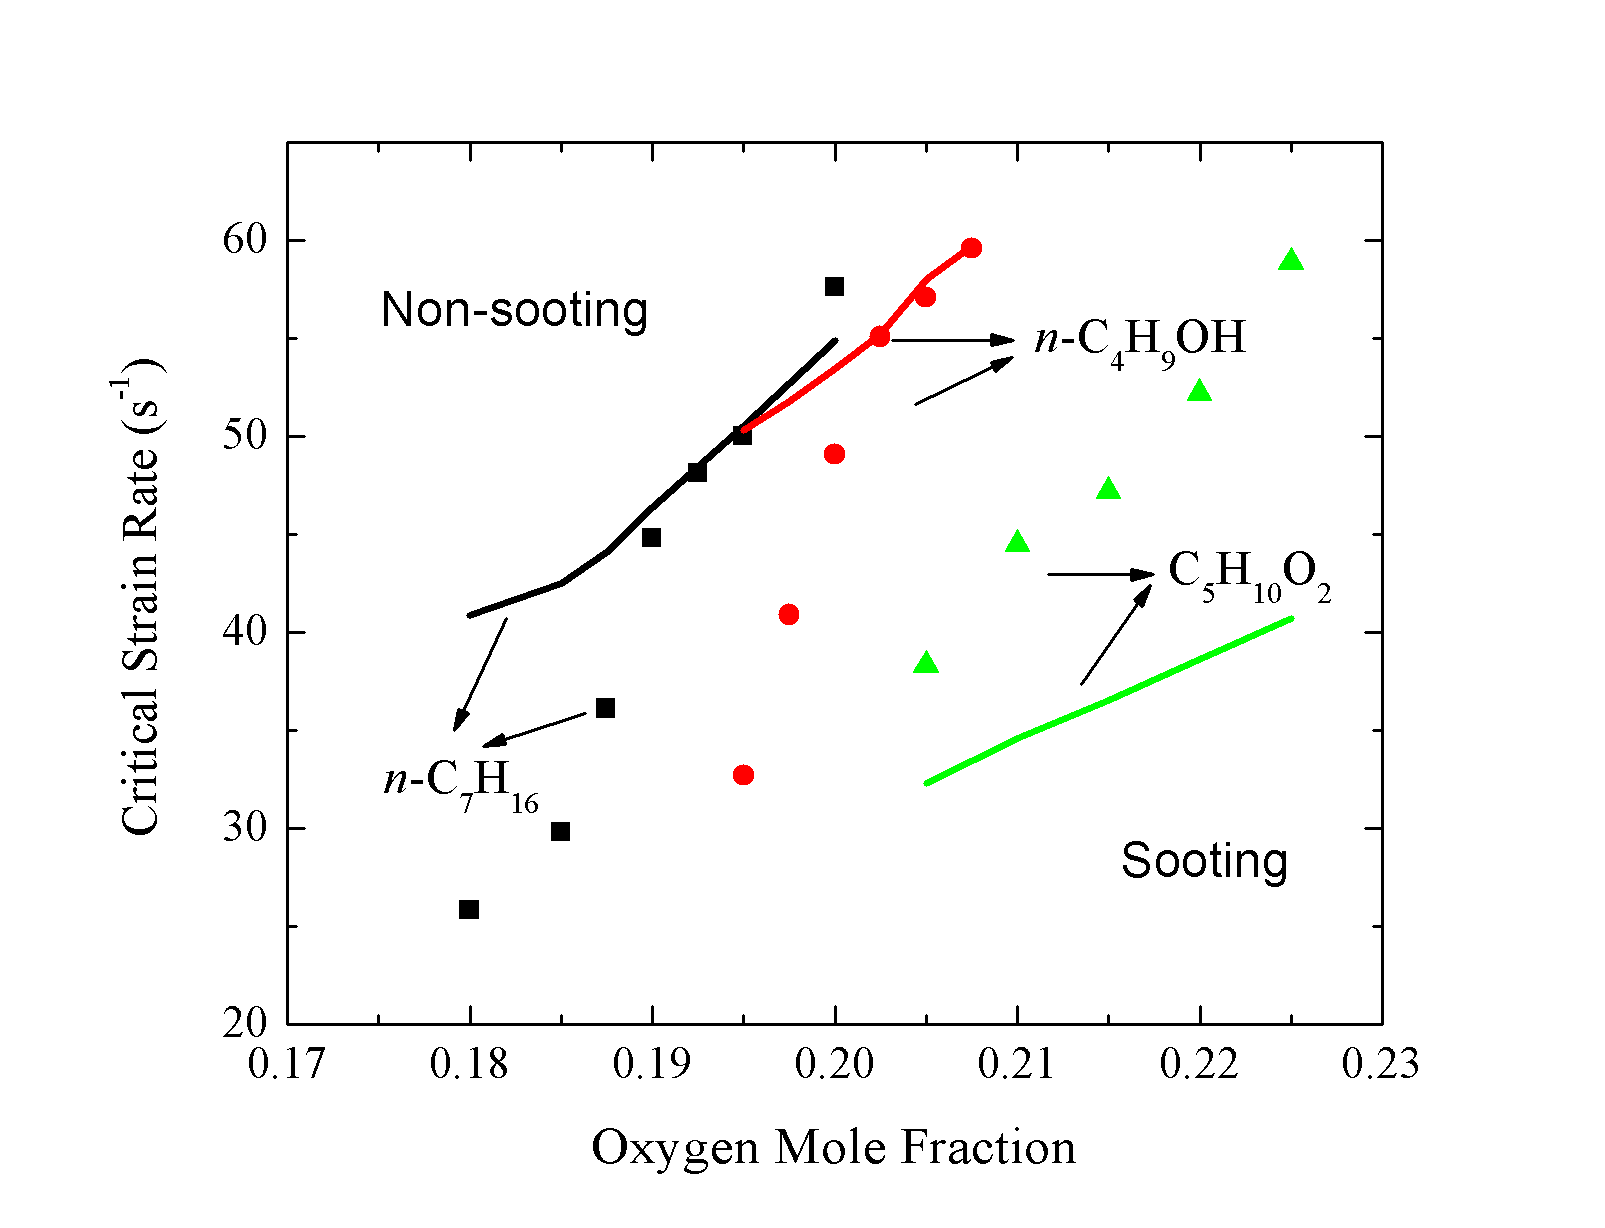
\includegraphics[width=0.48\textwidth]{Exp-Comp.png}
  \normalsize
  \vspace{-0.2in}
  \caption{Experimental (symbols) and computational (lines) CSRs. }
  \label{fig:Exp-Comp}
\end{figure}

To understand this discernible difference, sensitivity and reaction path analysis was performed on a representative PAH species, naphthalene (A2-C$_{10}$H$_8$). As shown in Fig.~\ref{fig:SA4} and Fig.~\ref{fig:Pathways_PAH}, in spite of different sooting propensities, the important PAH chemical pathways for the three fuels are essentially the same. Initially, fuel cracks to unsaturated C$_3$ to C$_5$ chains through H abstraction followed by $\beta$-scission reactions. These chain molecules further decompose to allyl radical (A-C$_3$H$_5$, CH$_2$=CH-CH$_2^*$) and propene (C$_3$H$_6$), which contribute to C$_5$ and C$_6$ ring formation by either combining with acetylene (C$_2$H$_2$) or forming propargyl (C$_3$H$_3$), which further combines with itself to form rings. Larger rings are formed by successive CH$_3$, C$_2$H$_2$ and C$_3$H$_3$ addition on phenyl (A1-) radicals. The C$_5$ ring combination and C$_9$ methyl addition reactions
\begin{align*}
  2 C_5H_5 &\Longleftrightarrow A2-C_{10}H_8 + 2 H\\
  C_9H_7 + CH_3 &\Longleftrightarrow A2-C_{10}H_8 + 2 H
\end{align*}
directly contribute to the formation of A2. 

\begin{figure}[ht]
  \centering
  \scriptsize
%  \vspace{-0.4in}
%  \hspace{-0.8in}
  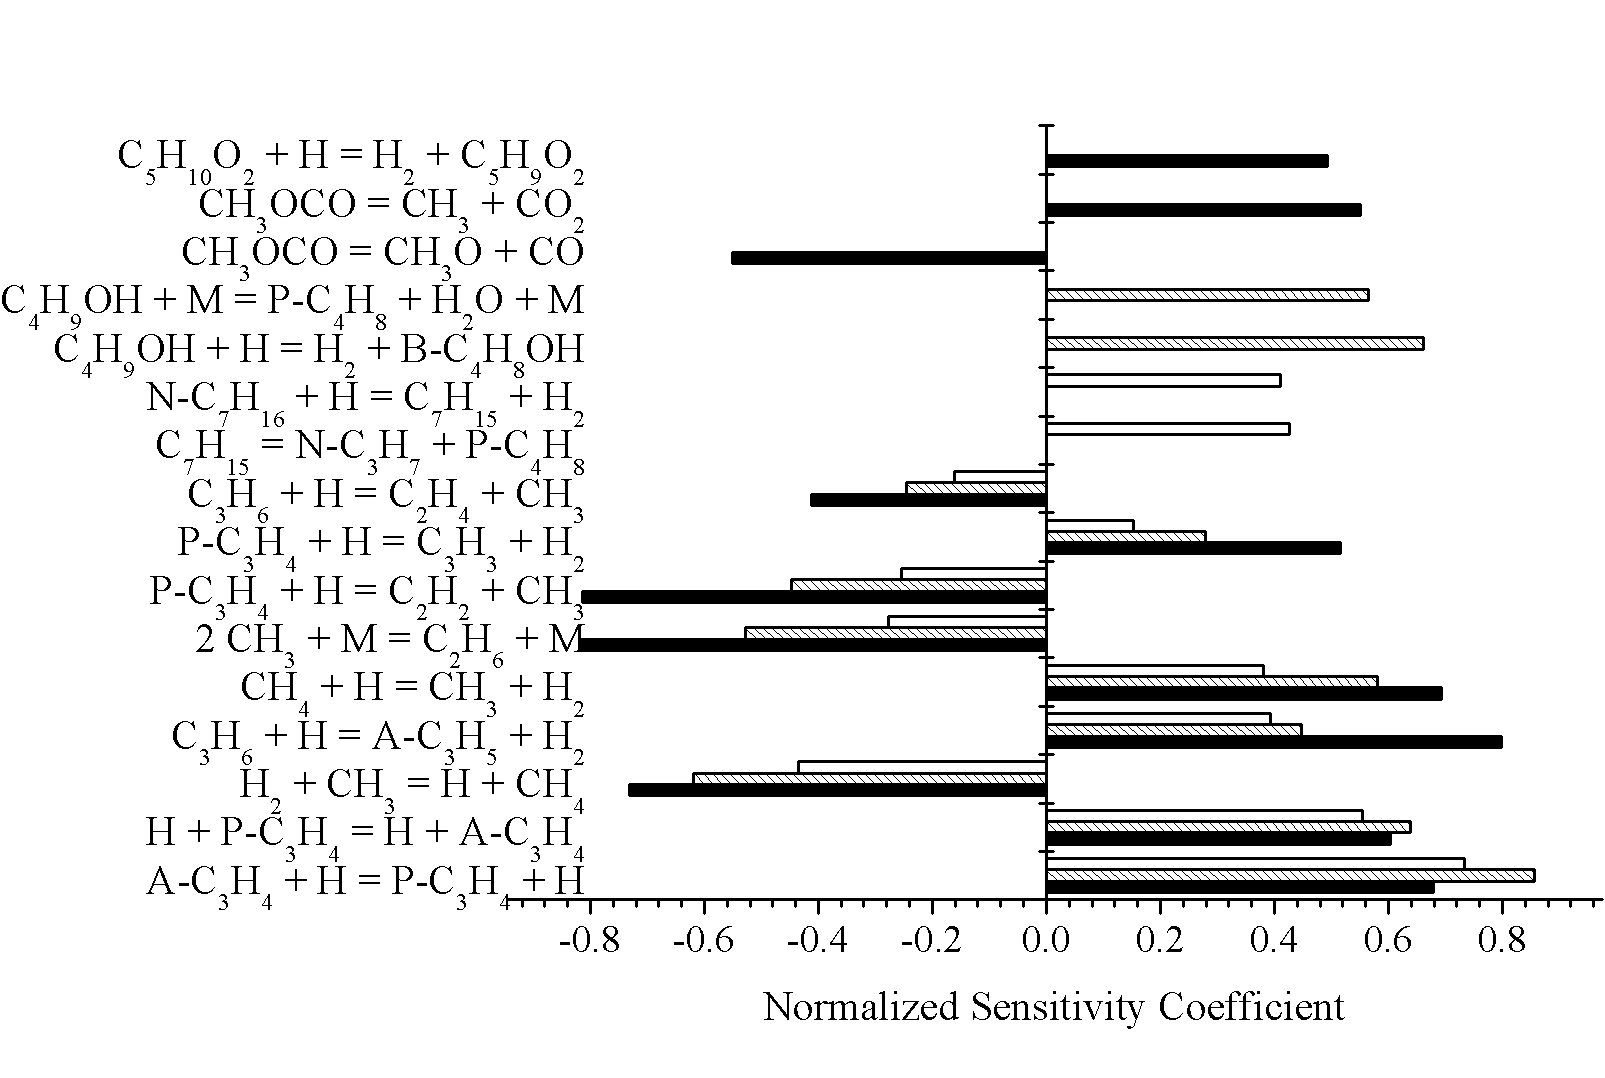
\includegraphics[trim=0mm 0mm 0mm 8mm, clip=true,width=0.49\textwidth]{Chain.png}
  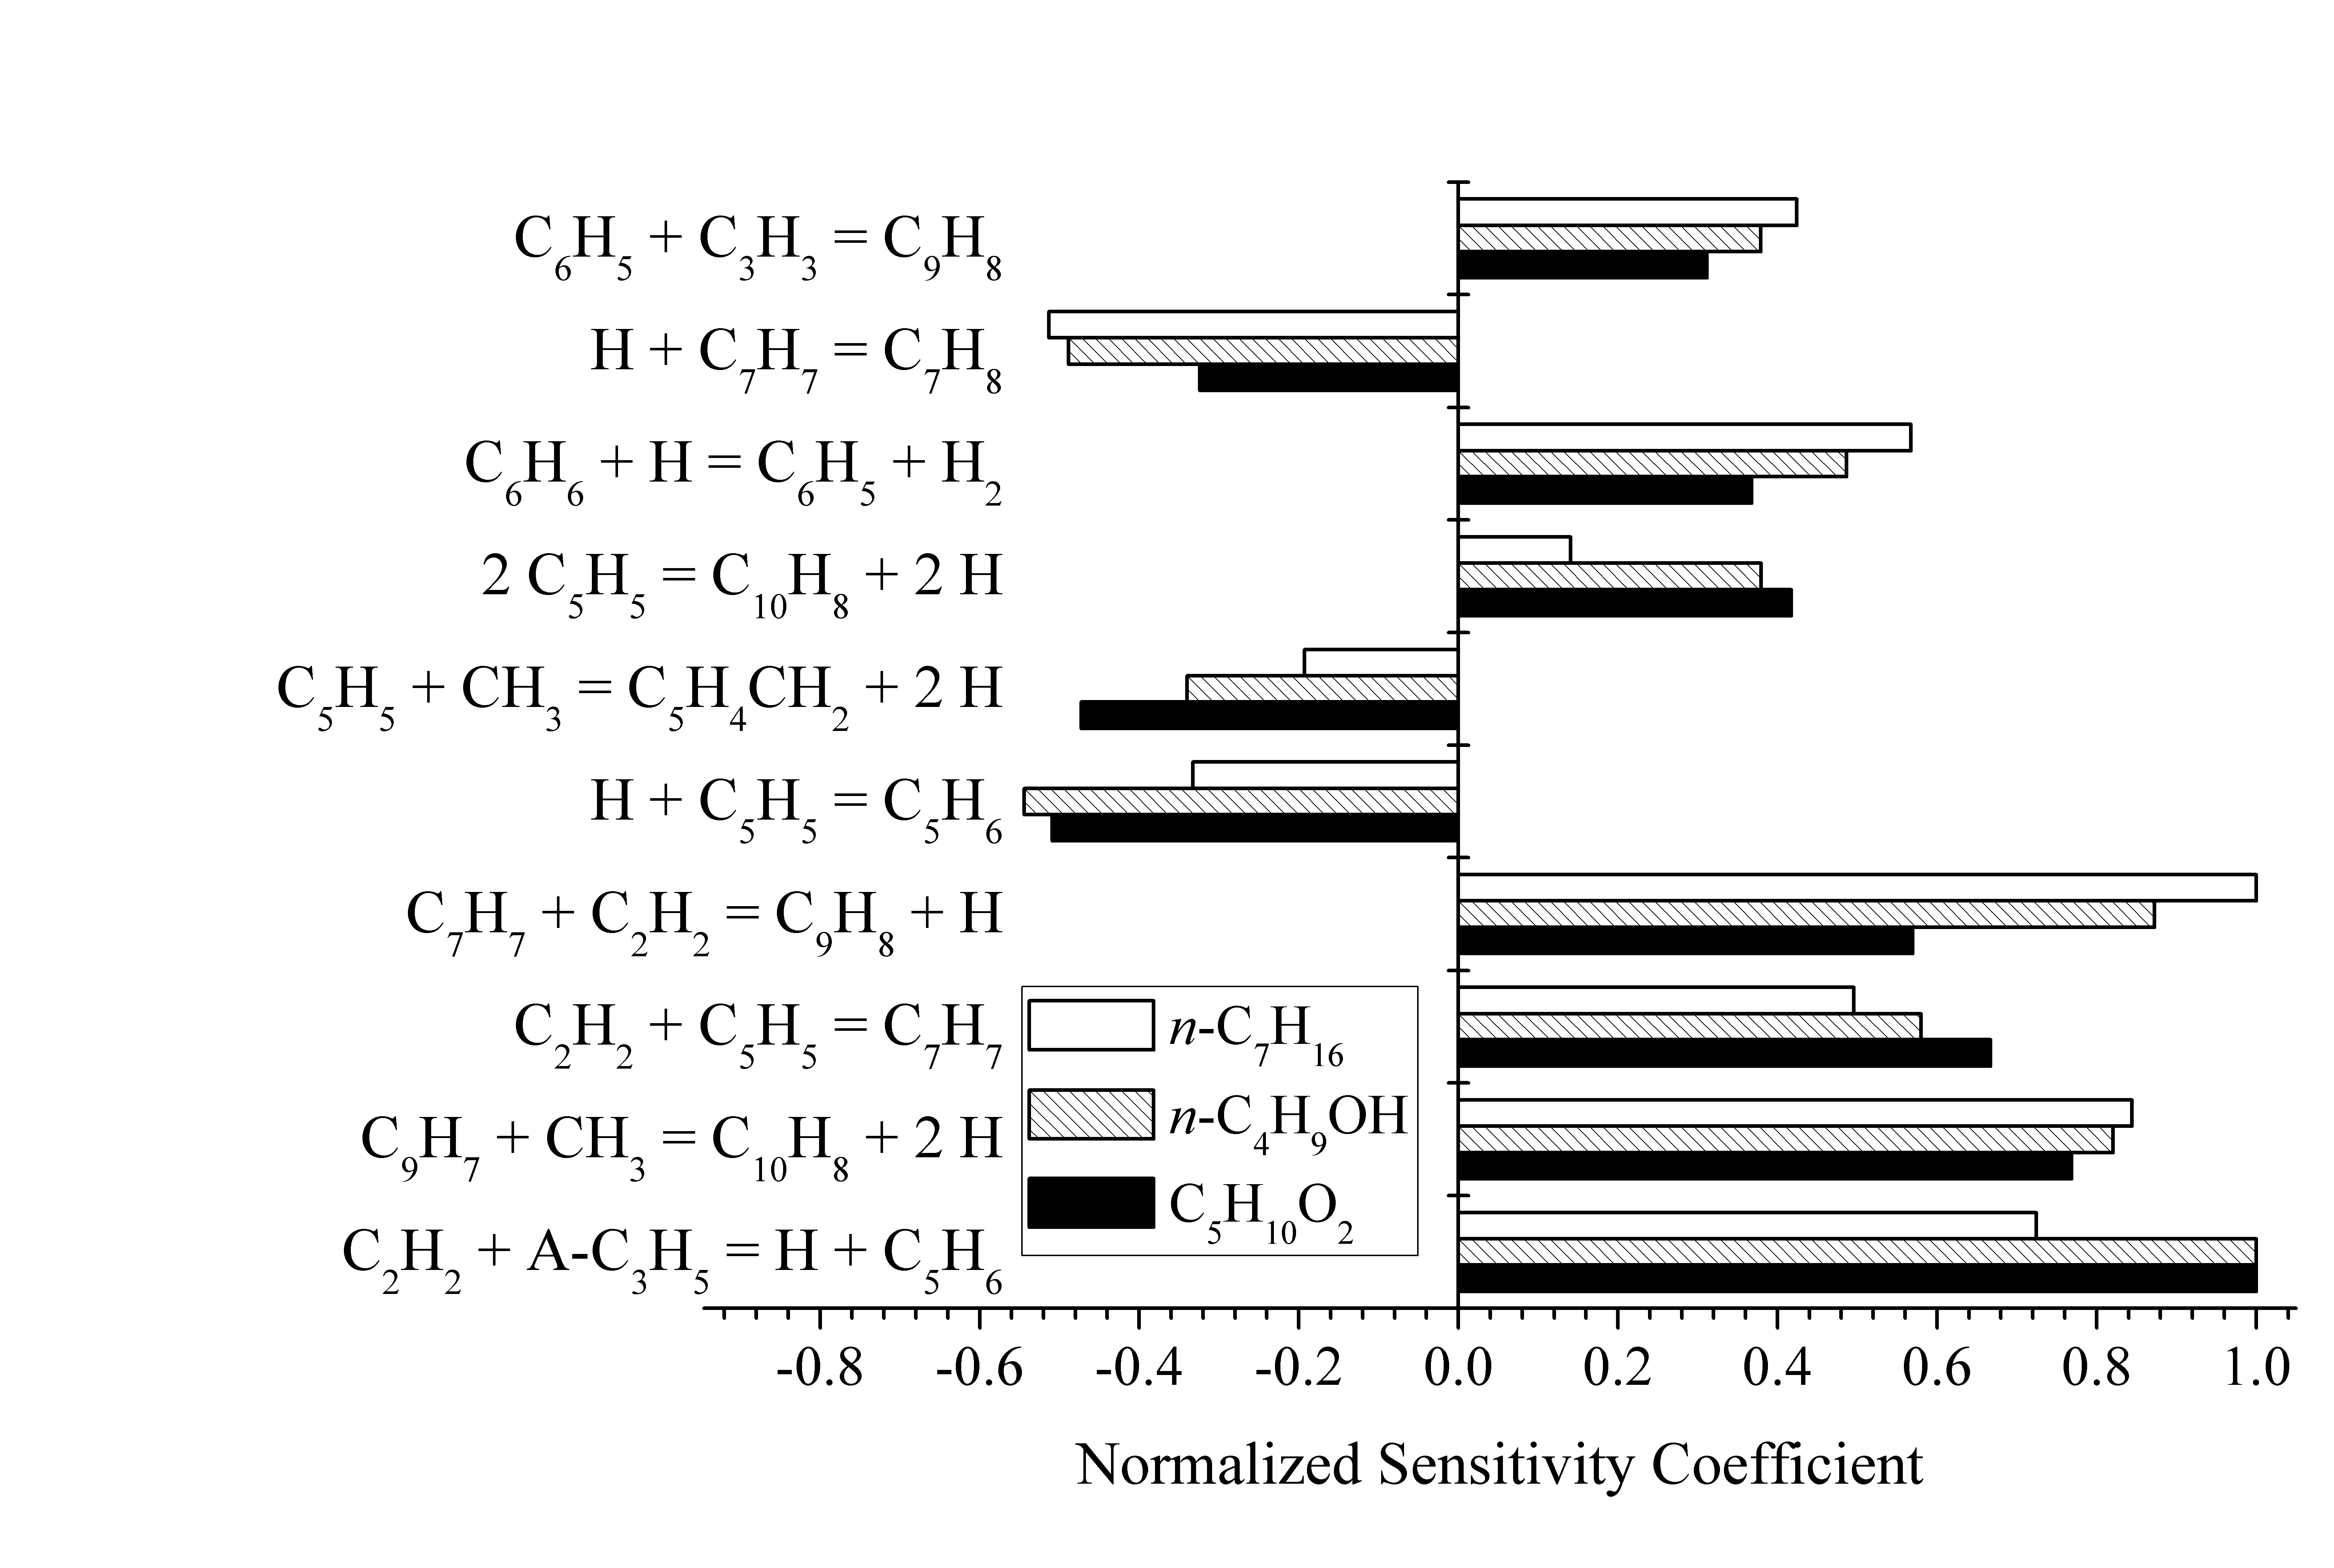
\includegraphics[trim=0mm 0mm 0mm 8mm, clip=true,width=0.49\textwidth]{Ring.png}
  \normalsize
  \vspace{-0.2in}
  \caption{Sensitivity of the maximum $Y_{A2}$ to kinetics at the strain rate of $16$ s$^{-1}$ and $X_{O_2}=0.2$. Left: Intermediate chain radical reactions. Right: Ring formation reactions.}
  \label{fig:SA4}
\end{figure}

Although the PAH pathways for the three fuels are similar, how soot precursors are formed from fuel cracking processes, and the relative importance of chemical pathways are fuel specific. Noting the similarity in the chemical pathways beyond A-C$_3$H$_5$ and C$_3$H$_6$, the fuel specific breakdown pathways that lead to the generation of these precursors are depicted in Fig.~\ref{fig:Pathways_Fuel}. For both $n$-heptane and $n$-butanol, butene (P-C$_4$H$_8$) is formed from the fuel decomposition, which contributes to $25\%$ of A-C$_3$H$_5$ production, and is strongly promoting A2 formation, according to the sensitivity analysis. Moreover, the fuel bound oxygen in $n$-butanol turns into water during this intramolecular water elimination reaction, rather than contributes to carbon reduction~\cite{mcenally05,mcenally11}, which explains the similar sooting behavior as $n$-heptane. On the other hand, C$_3$ species are the largest species formed from methyl butanoate cracking, due to the fuel bound oxygen. As pointed out in Ref.~\cite{westbrook06}, the double C=O bond is very difficult to break, such that the carbon chain length is reduced when C-C bond is broken due to $\beta$-scission. The oxygenated parts are then oxidized to CO and CO$_2$, preventing the carbon from entering the pool for soot formation~\cite{feng12,wangyl11}. In Fig.~\ref{fig:SA4}, it further shows that when two oxygen atoms in CH$_3$OCO keeps attaching to different carbon atoms, it is more efficient to demote A2 formation. Due to the reduction in A-C$_3$H$_5$ precursors from methyl butanoate decomposition, both A-C$_3$H$_5$ and C$_5$H$_5$ concentrations are lower than the other fuels, as shown in Fig.~\ref{fig:CxHy}, such that the A2 formation is less sensitive to the C$_5$ pathway, as the reaction rate depends quadratically on the C$_5$H$_5$ concentration. This reduction in soot precursors from fuel cracking processes distinguishes methyl butanoate from $n$-heptane and $n$-butanol, in terms of the sooting propensity.

\begin{figure*}[h]
  \centering
  \scriptsize
%  \vspace{-0.4in}
%  \hspace{-0.4in}
  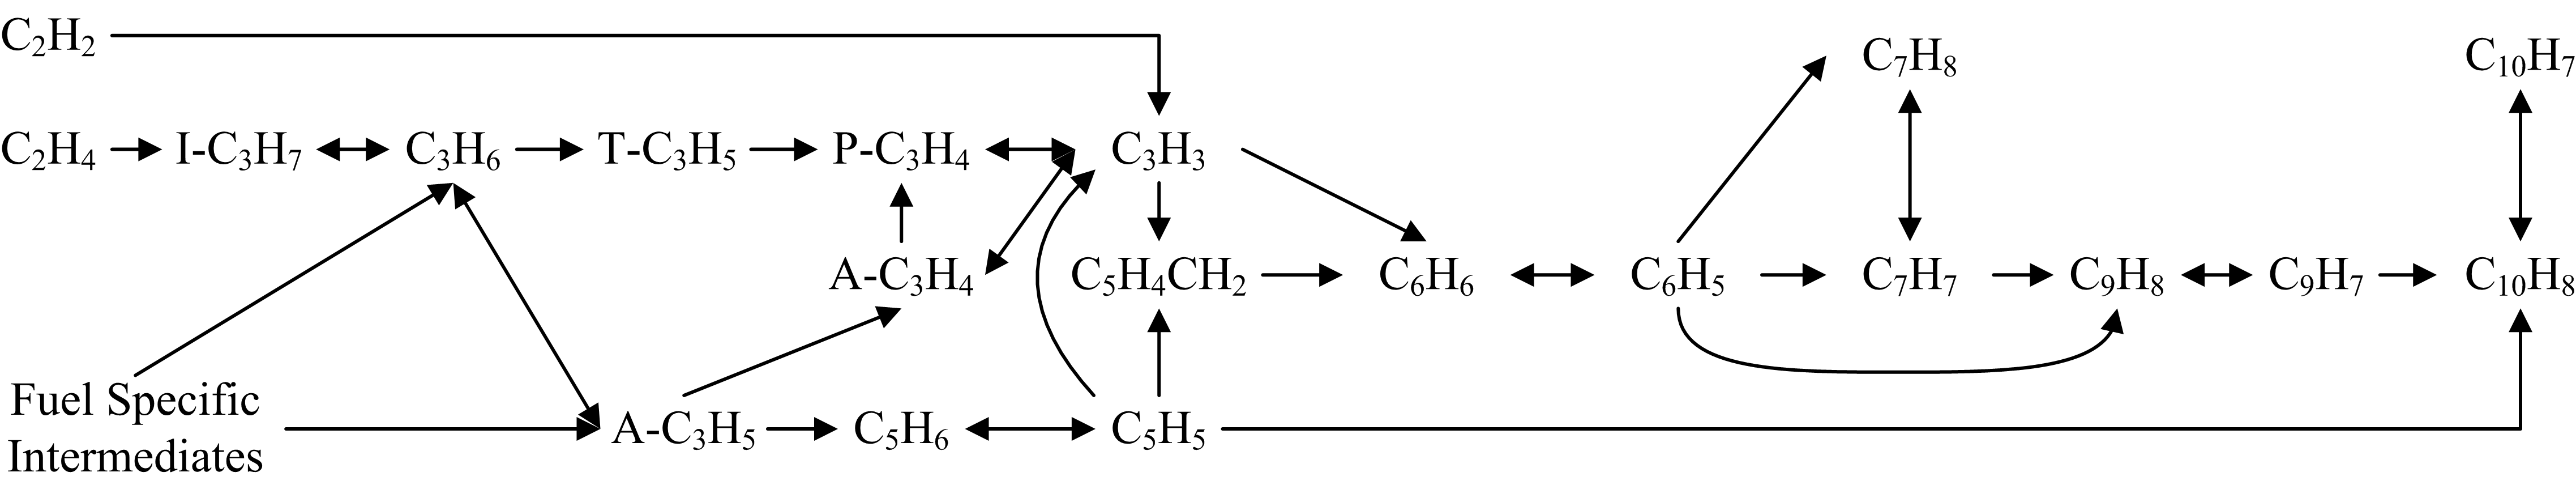
\includegraphics[width=1.0\textwidth]{Pathways-PAH.png}
  \normalsize
  \caption{Chemical pathways for A2 formation at the strain rate of $16$ s$^{-1}$ and $X_{O_2}=0.2$.}
  \label{fig:Pathways_PAH}
\end{figure*}

\begin{figure*}[h]
  \centering
  \scriptsize
%  \vspace{-0.4in}
%  \hspace{-0.4in}
  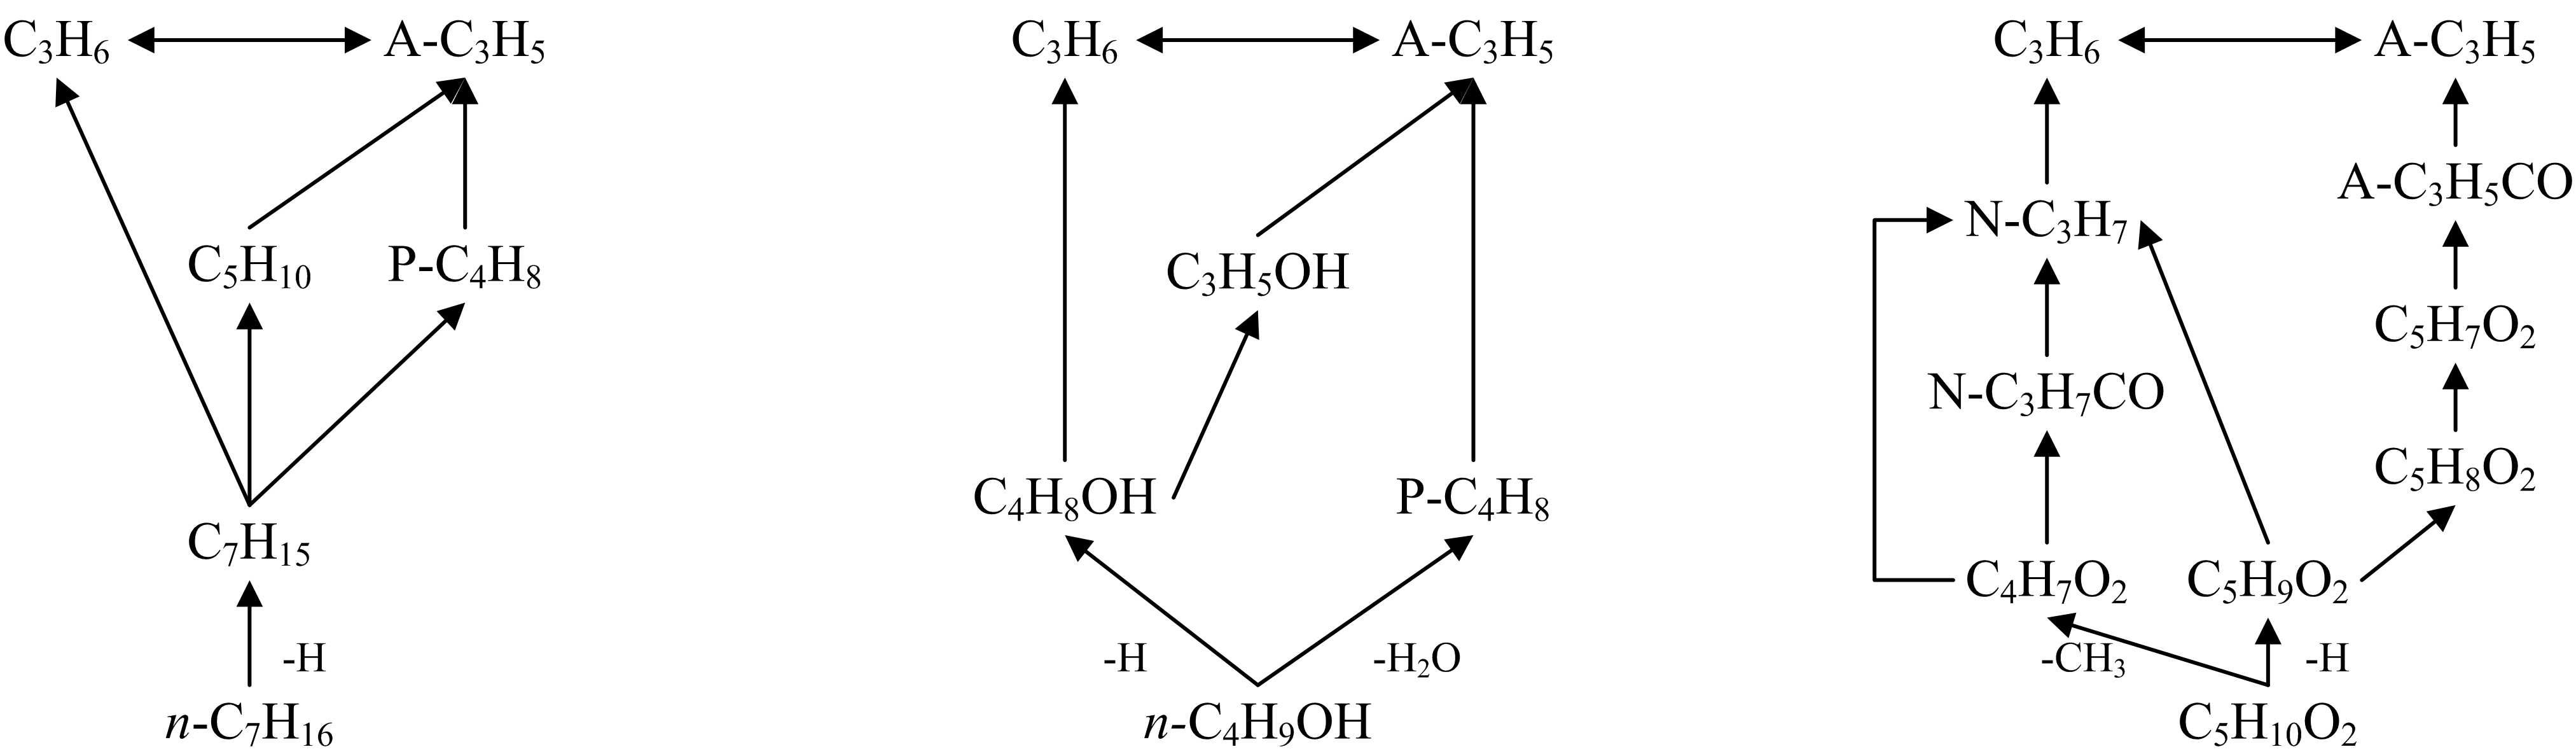
\includegraphics[width=1.0\textwidth]{Pathways_Fuel.png}
  \normalsize
  \caption{Fuel specific pathways for C$_3$H$_6$ and A-C$_3$H$_5$ formation at the strain rate of $16$ s$^{-1}$ and $X_{O_2}=0.2$. From left to right: $n$-heptane, $n$-butanol and methyl butanoate.}
  \label{fig:Pathways_Fuel}
\end{figure*}
At this point, we have identified pathways and species that are responsible for soot formation. The next question that naturally arises is how sensitive they are to the increasing strain rate that leads to reduced soot formation. To answer this question, integrated $f_V$ under various strain rates and $f_V$ profiles for low and critical strain rate cases were presented in Fig.~\ref{fig:fv-SR-combo}. All profiles shift in the direction of the liquid pool as higher flow rate pushes the stagnation plane further towards the pool. As expected, sooting propensities drop due to reduced residence time, and methyl butanoate is the least sooty, while $n$-butanol is overall as sooty as $n$-heptane. Although not shown here, sensitivity and reaction path analysis were conducted and no substantial difference was found compared with low strain rate cases. As the CSR was measured and defined based on the absolute value of $f_V$, it is reasonable to anticipate a lower CSR for methyl butanoate, since it is the least sooty fuel even at lower strain rates. However, if the CSR is defined based on a relative metric, in other words, to be the strain rate at which the $f_V$ is $10\%$ of the value at a fixed low strain rate ($16$ s$^{-1}$), the three fuels are very close, which indicates the potential similarity in rate limiting steps of the soot formation.

\begin{figure*}[h]
  \centering
  \scriptsize
%  \vspace{-0.4in}
%  \hspace{-0.4in}
  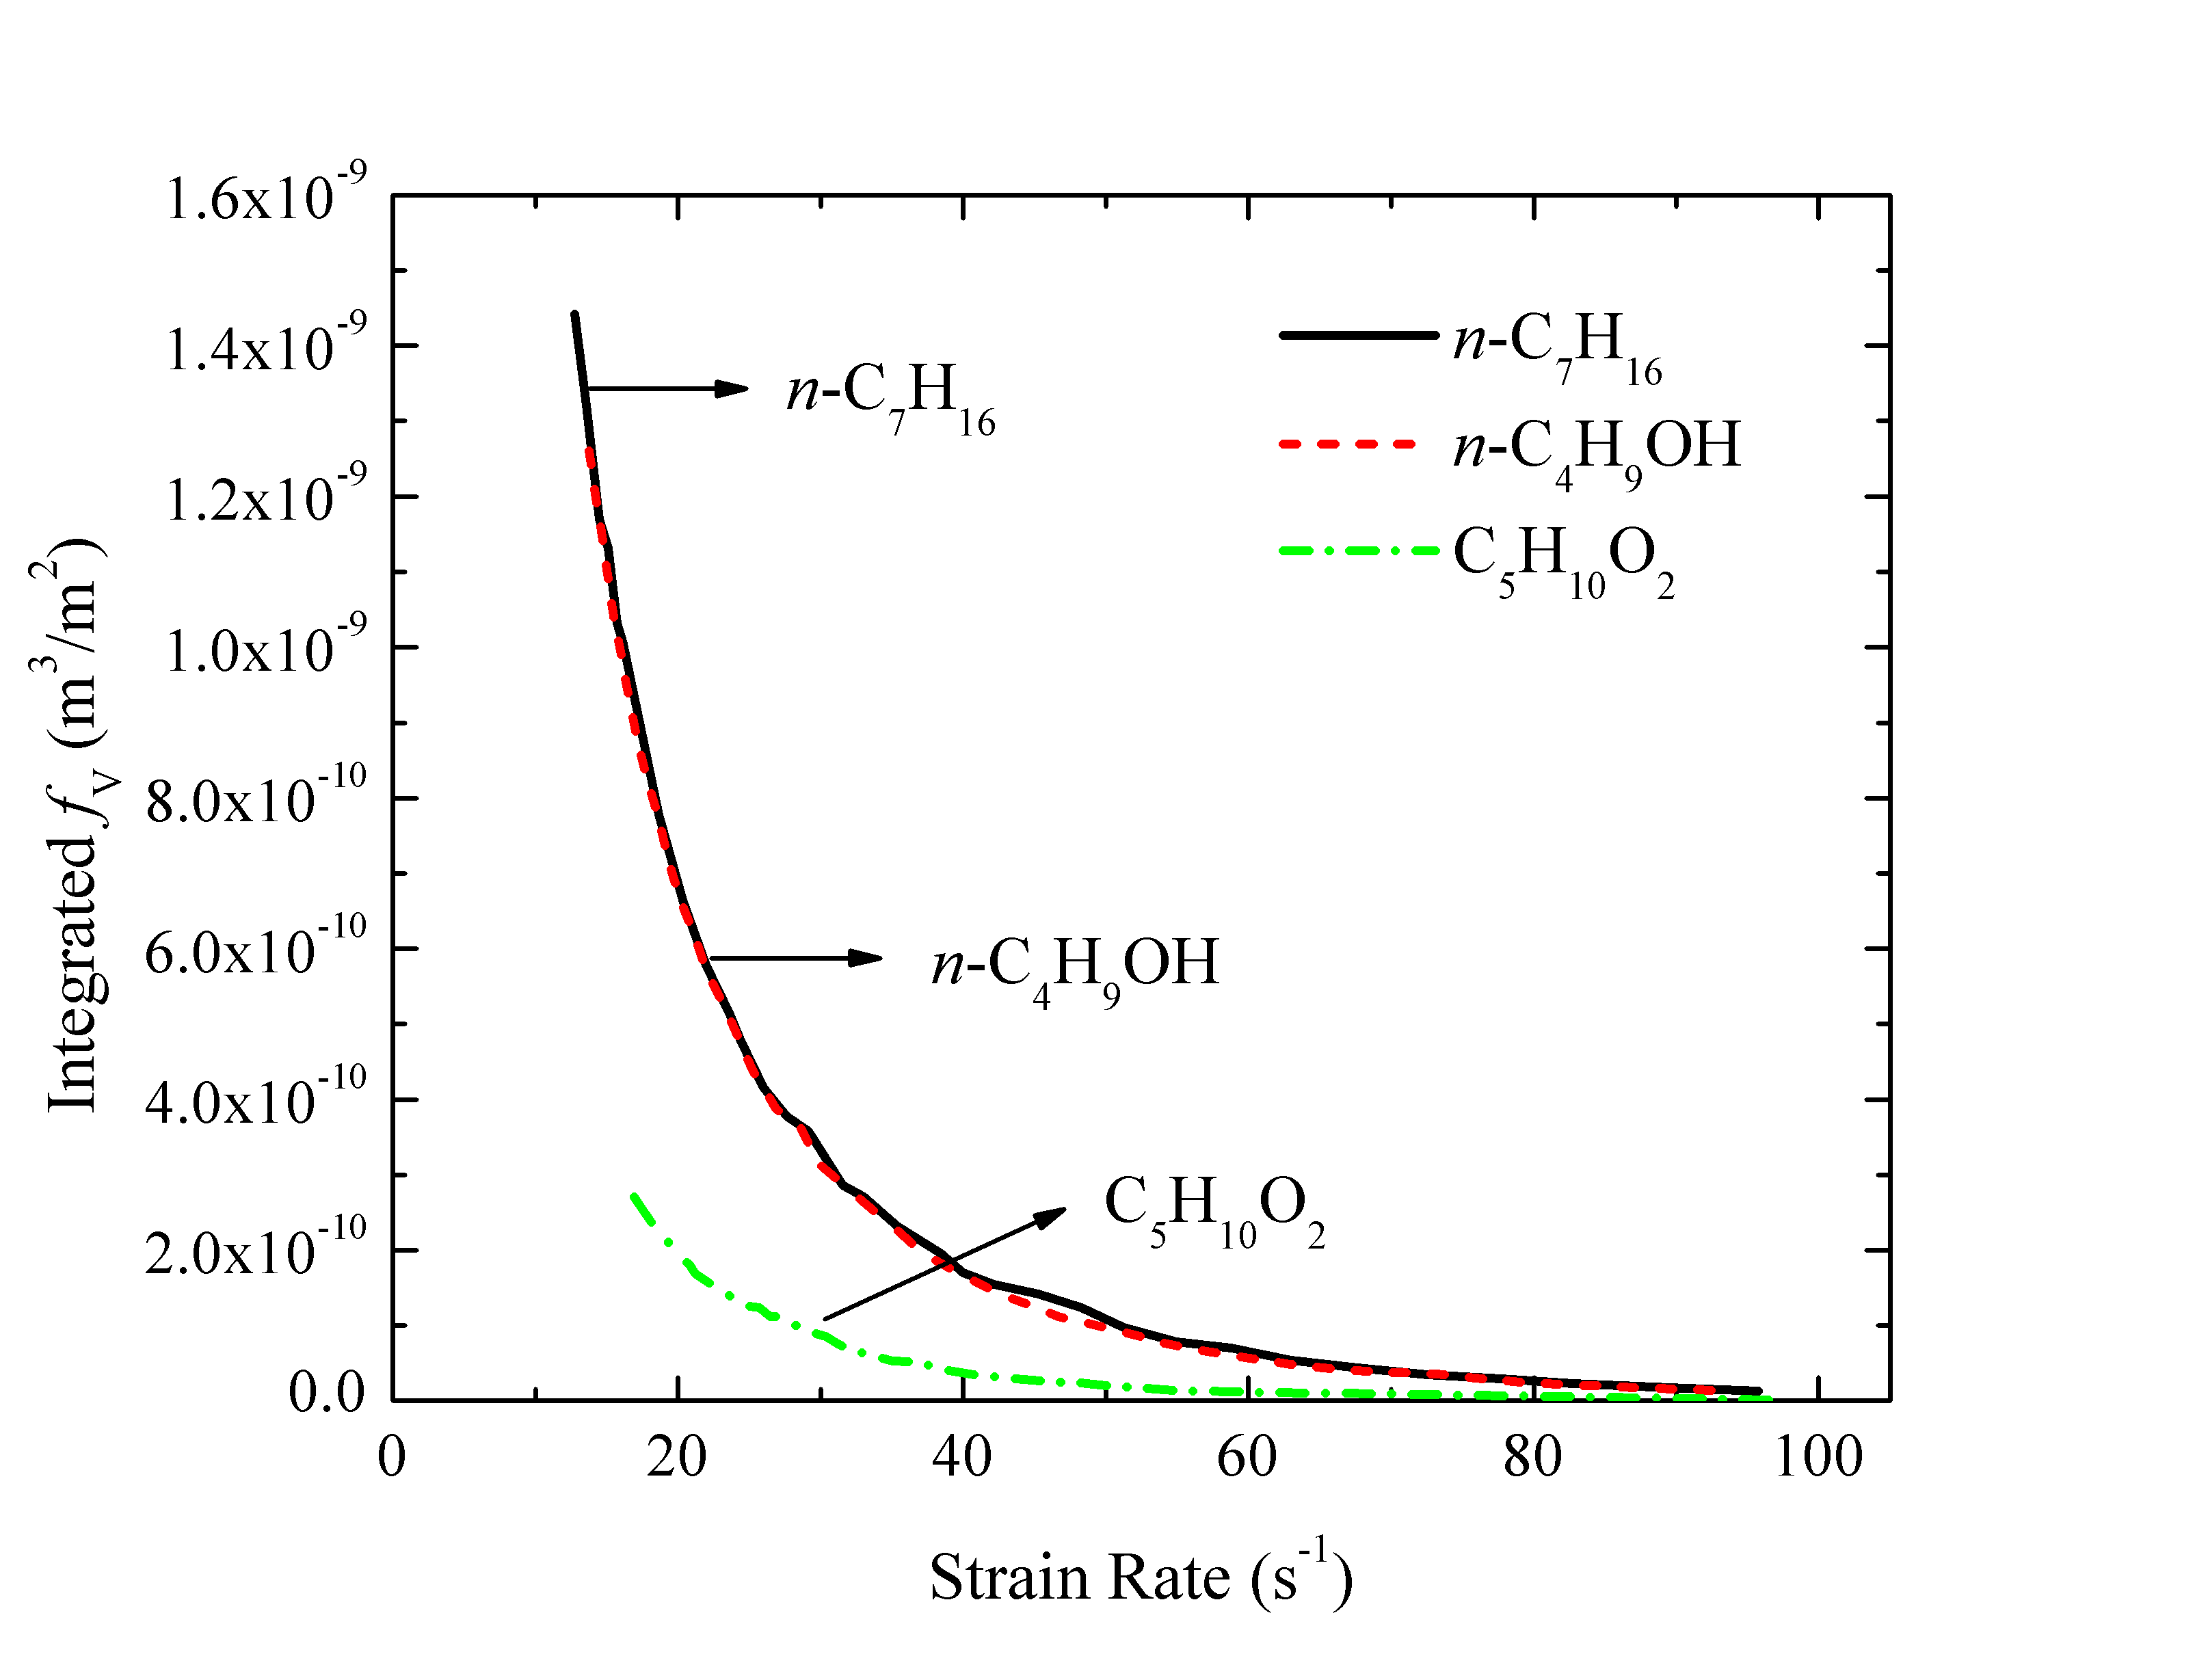
\includegraphics[trim=4mm 8mm 30mm 20mm, clip=true, width=0.48\textwidth]{SV-SR.png}
  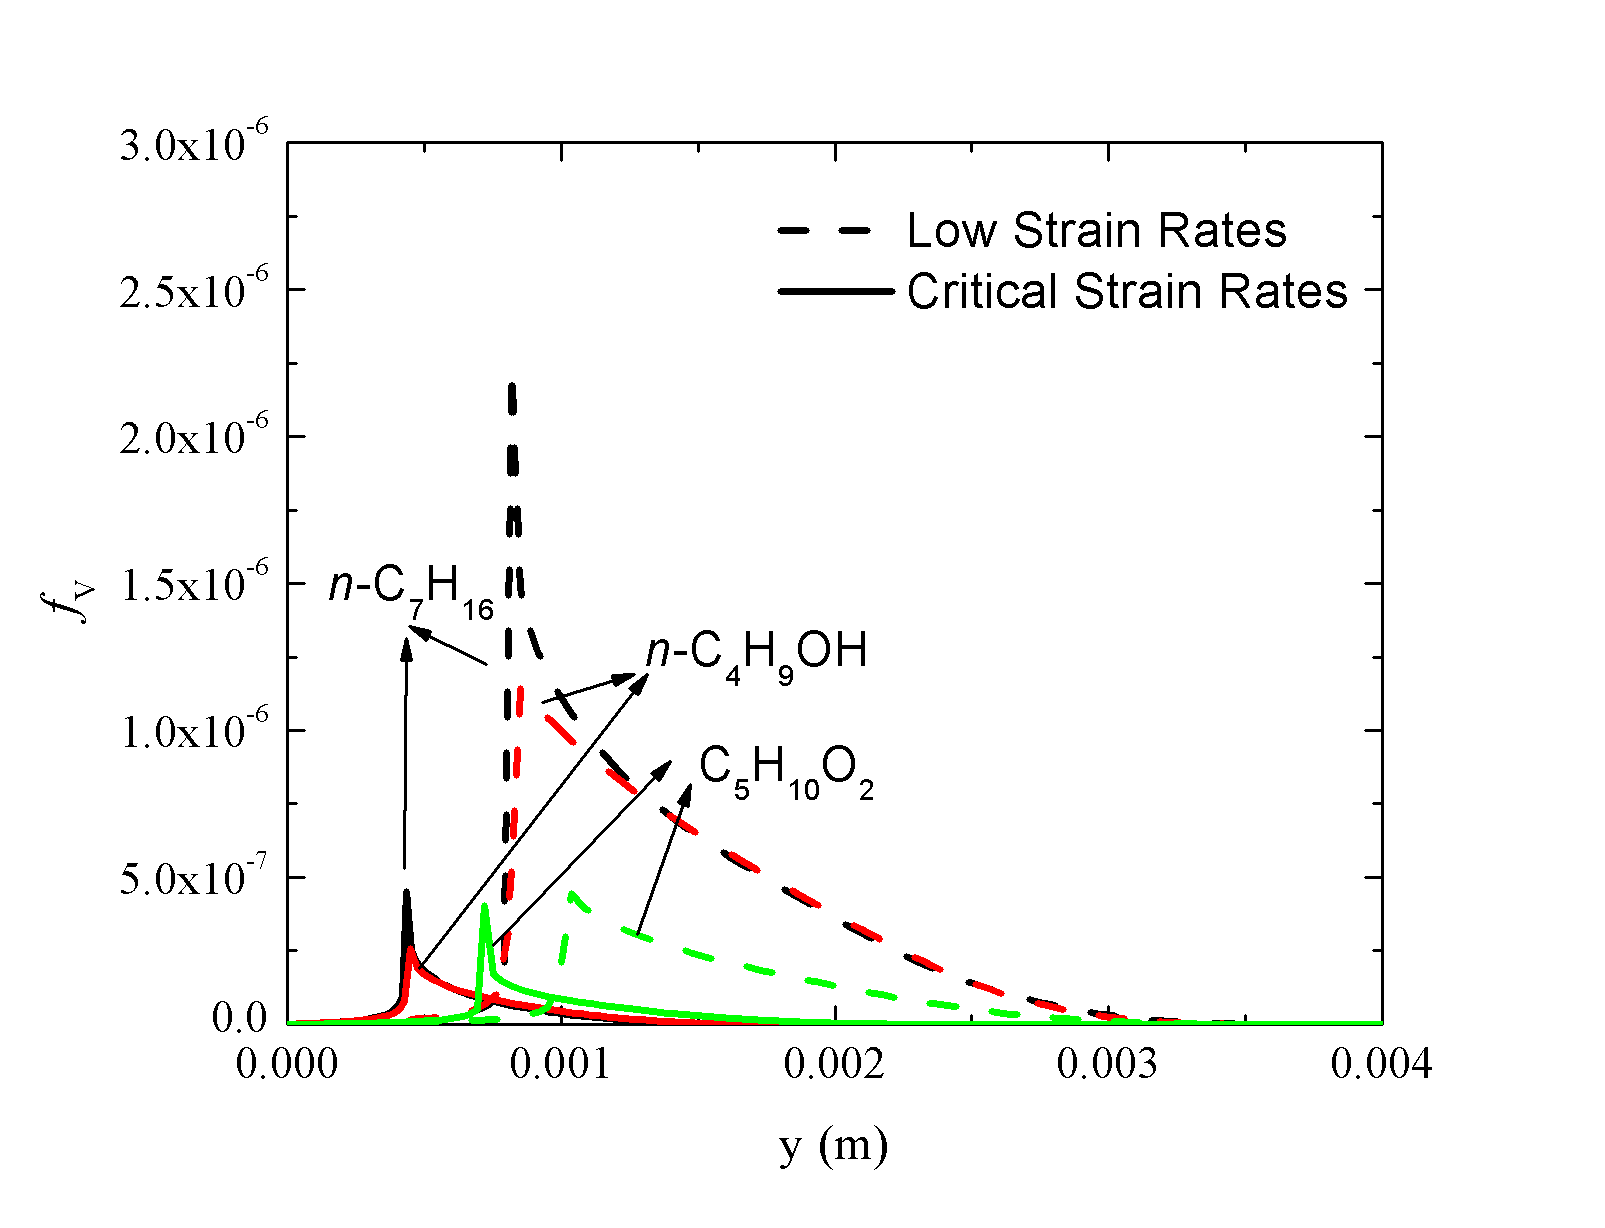
\includegraphics[trim=4mm 8mm 30mm 20mm, clip=true, width=0.48\textwidth]{fv-y.png}
  \normalsize
  \vspace{-0.2in}
  \caption{The responses of $f_V$ to strain rates at $X_{O_2}=0.2$. Left: $f_V$ integrated along the center axis of the stagnation-flow field. Right: $f_V$ profiles at low strain rates ($16$ s$^{-1}$) and CSRs.}
  \label{fig:fv-SR-combo}
\end{figure*}

To elucidate the rate limiting step, profiles of soot precursors at low and critical strain rates were compared with that of the $f_V$. Species with ring structures, namely C$_5$H$_6$, A1, C$_9$H$_8$, and A2, all respond similarly as $f_V$. However, this similarity is not retained when traced back to the upstream soot precursors, A-C$_3$H$_5$ and C$_3$H$_3$, as shown in Fig.~\ref{fig:CxHy}. Compared with the C$_5$ and C$_9$ ring structures, which have lower concentrations at CSR, these C$_3$ intermediates accumulate even higher concentrations, indicating that less of these species are involved in the ring formation relative to lower strain rate cases, which results in the soot reduction. Now it is clear that for all three fuels, these C$_3$ species play an essential role in current study, as it serves as the backbone of PAH precursors. In addition, the ring formation reactions 
\begin{align*}
  C_2H_2 + A-C_3H_5 &\Longleftrightarrow H + C_5H_6\\
  2 C_3H_3 &\Longleftrightarrow C_5H_4CH_2\\
  2 C_3H_3 &\Longleftrightarrow A1-C_6H_6
\end{align*}
are the rate limiting steps that are responsible for the critical strain rates.


\begin{figure*}[h]
  \centering
  \scriptsize
%  \vspace{-0.4in}
%  \hspace{-0.4in}
%  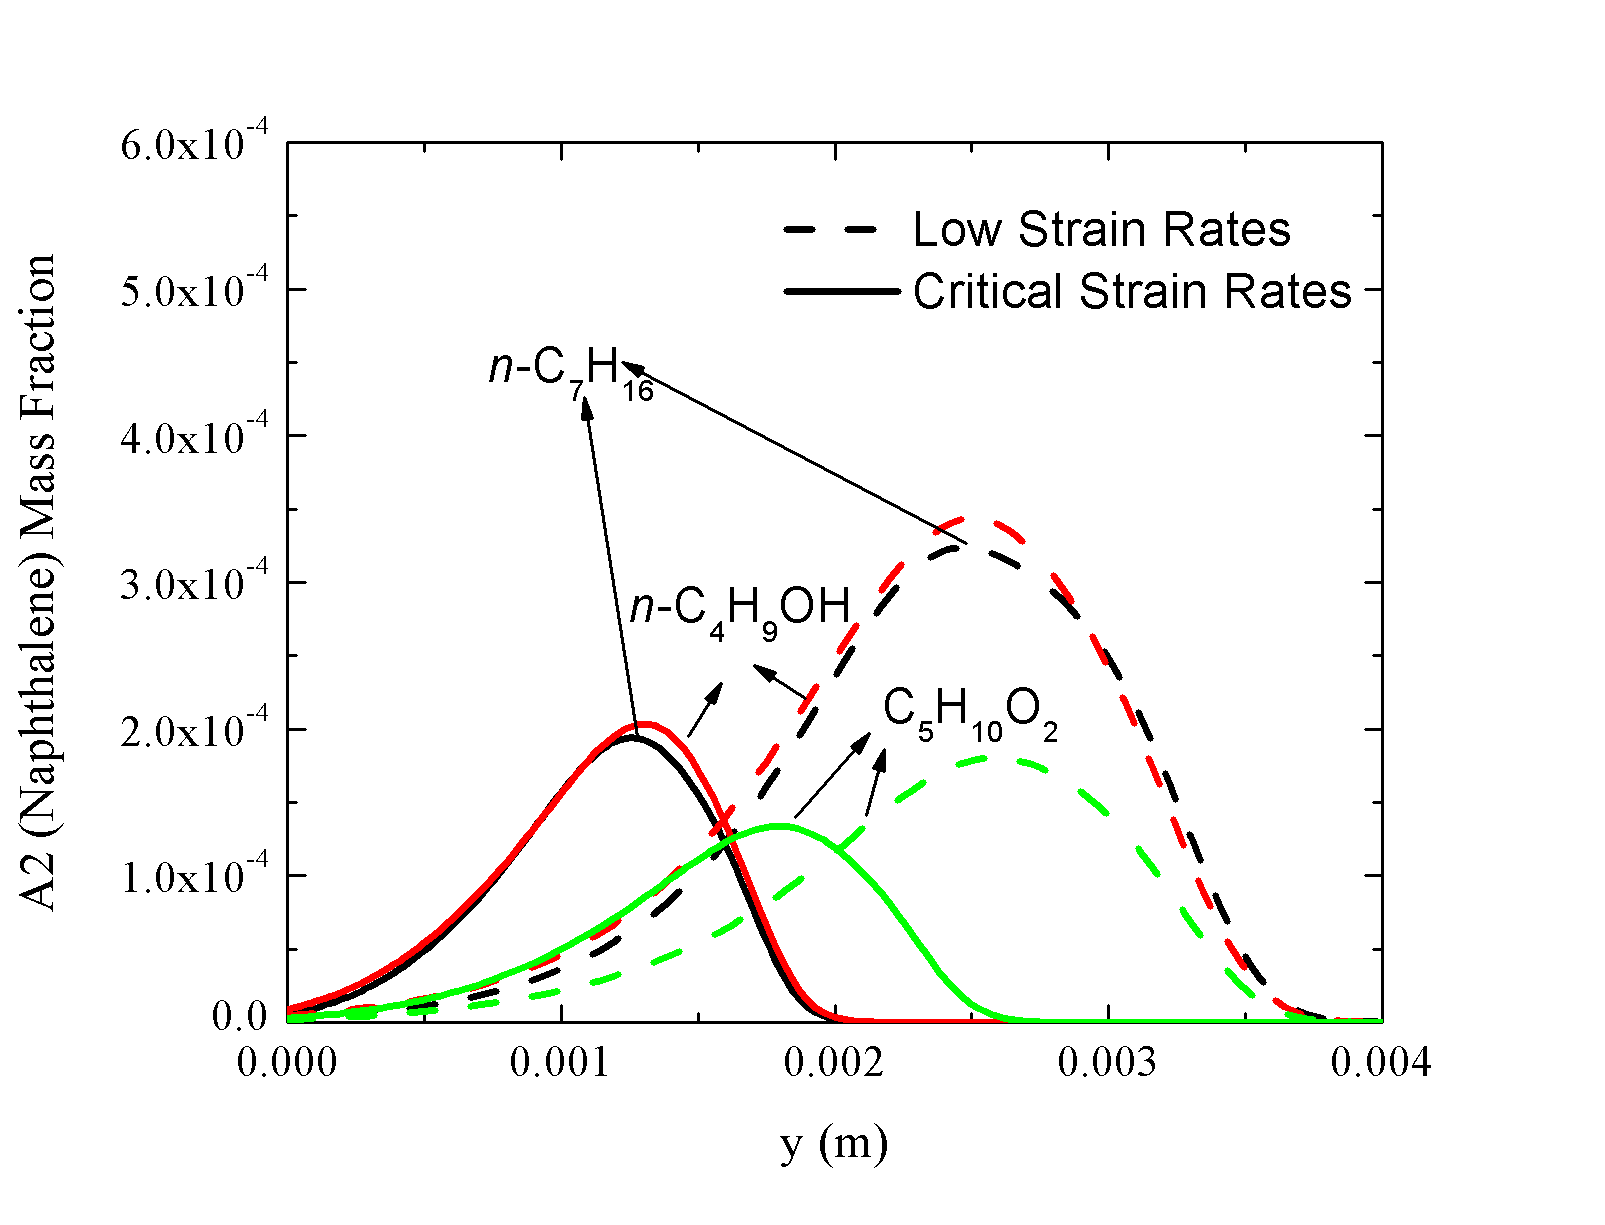
\includegraphics[trim=4mm 8mm 30mm 20mm, clip=true, width=0.48\textwidth]{A2-y.png}
%  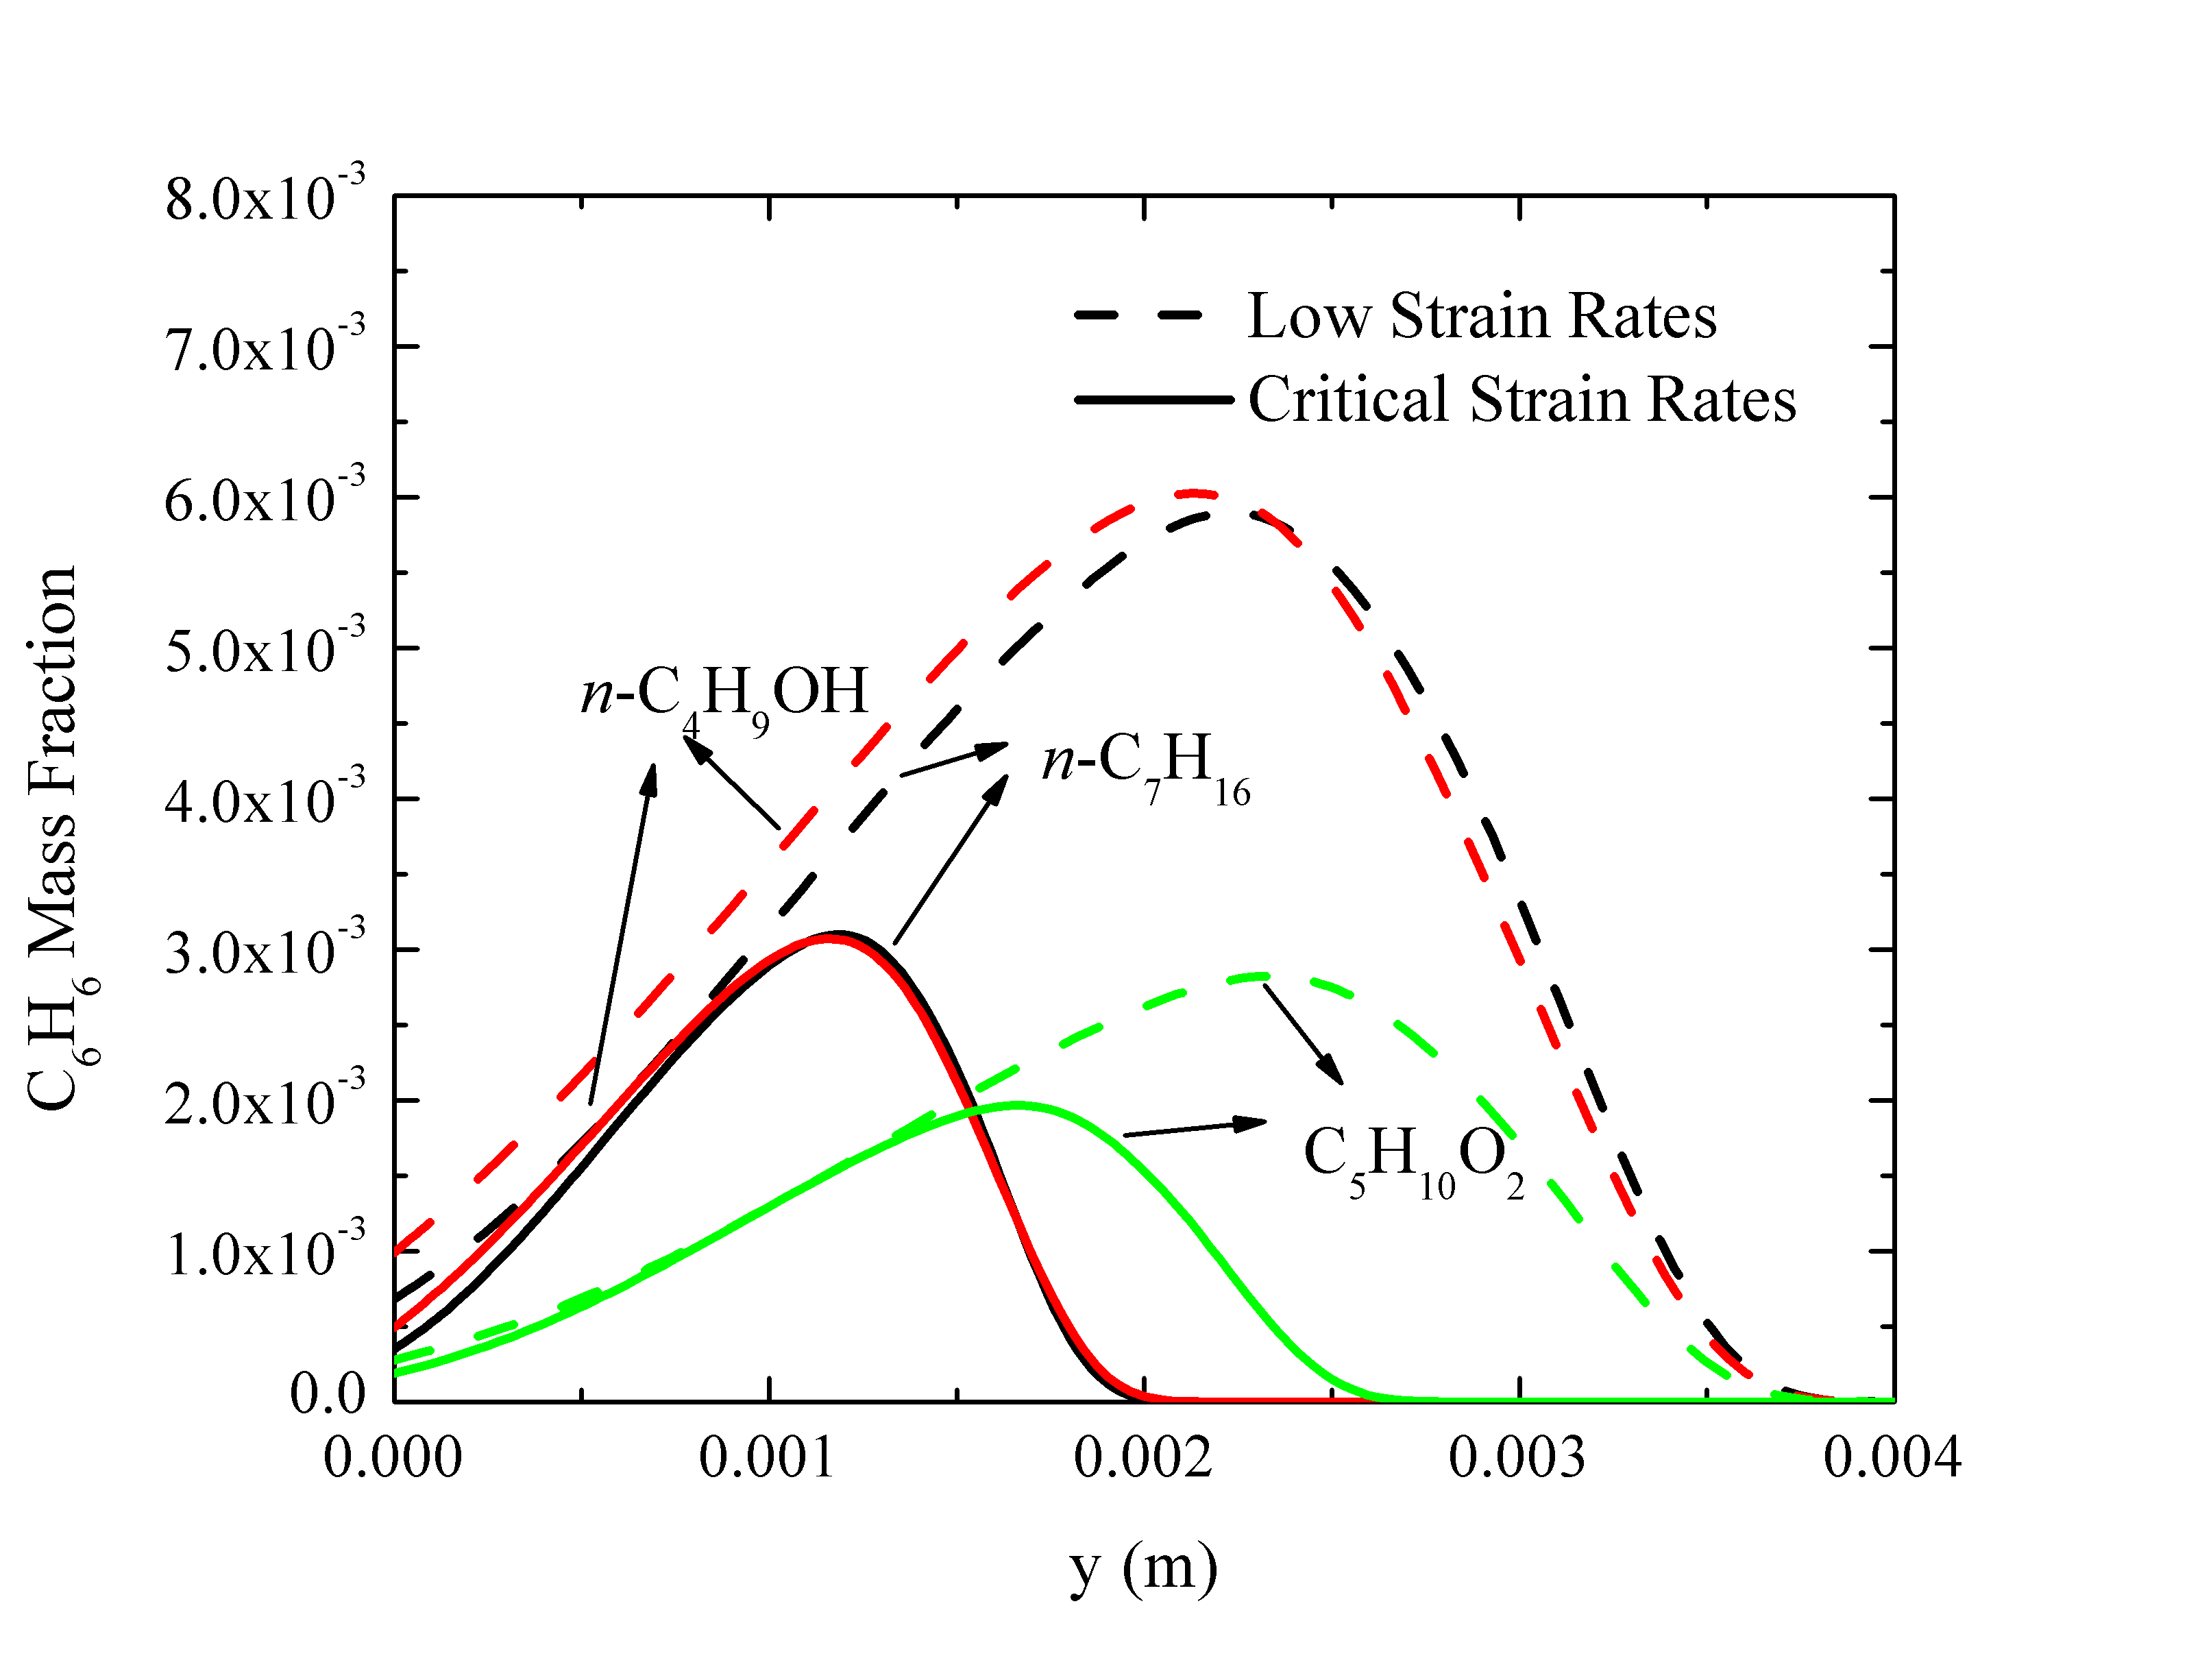
\includegraphics[trim=4mm 8mm 30mm 20mm, clip=true, width=0.48\textwidth]{A1-y.png}
%  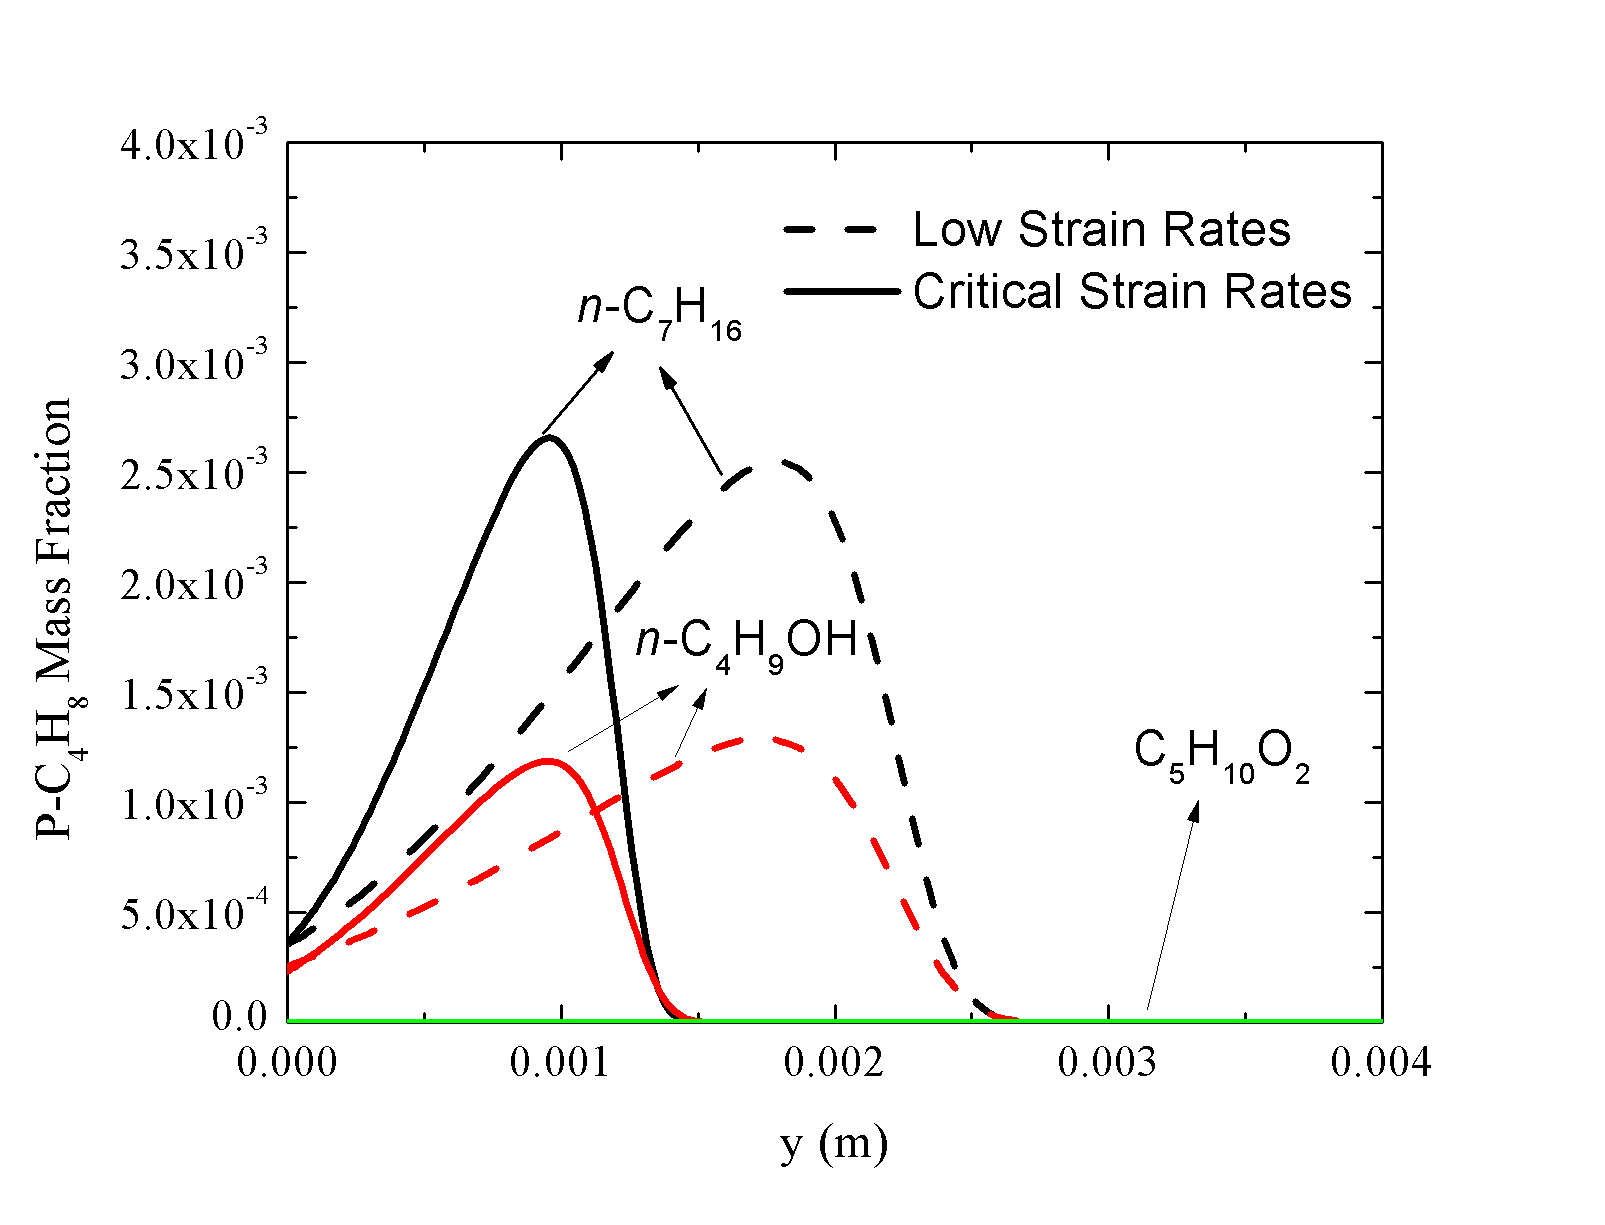
\includegraphics[trim=4mm 8mm 30mm 20mm, clip=true, width=0.48\textwidth]{P-C4H8-y.png}
%  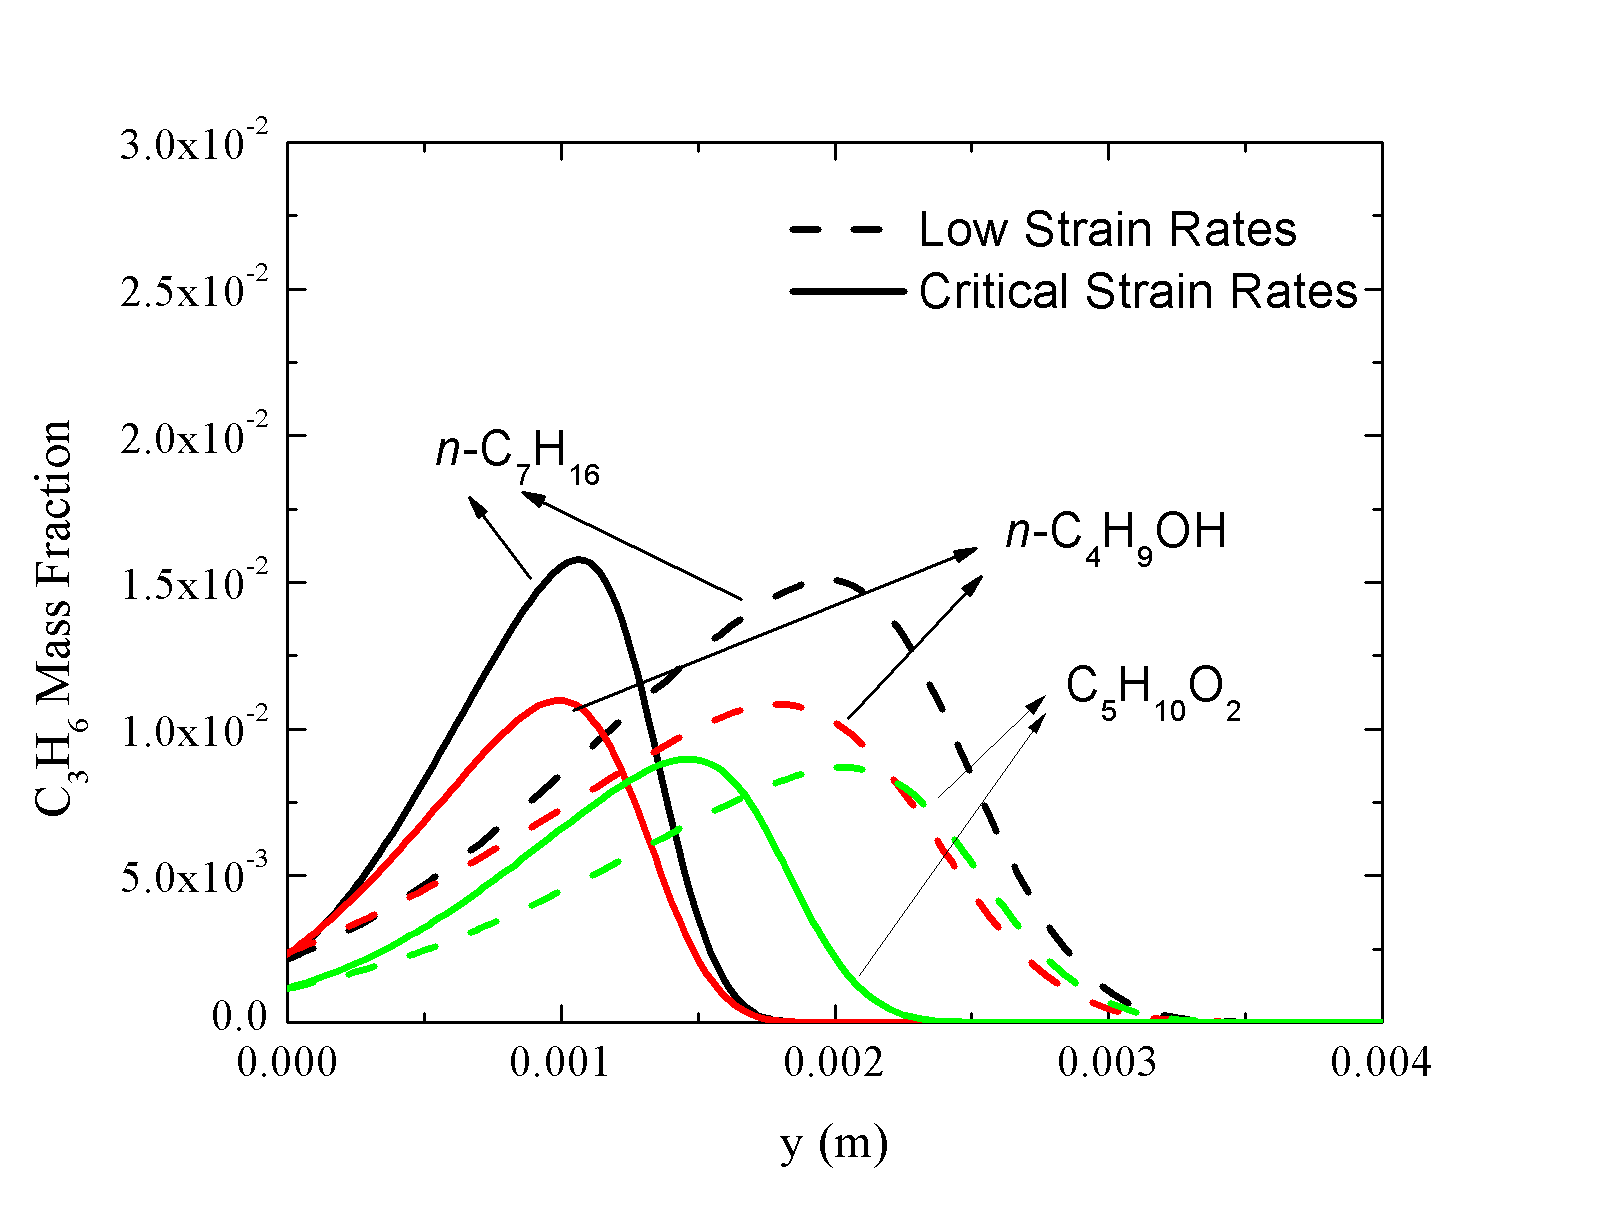
\includegraphics[trim=4mm 8mm 30mm 20mm, clip=true, width=0.48\textwidth]{C3H6-y.png}
  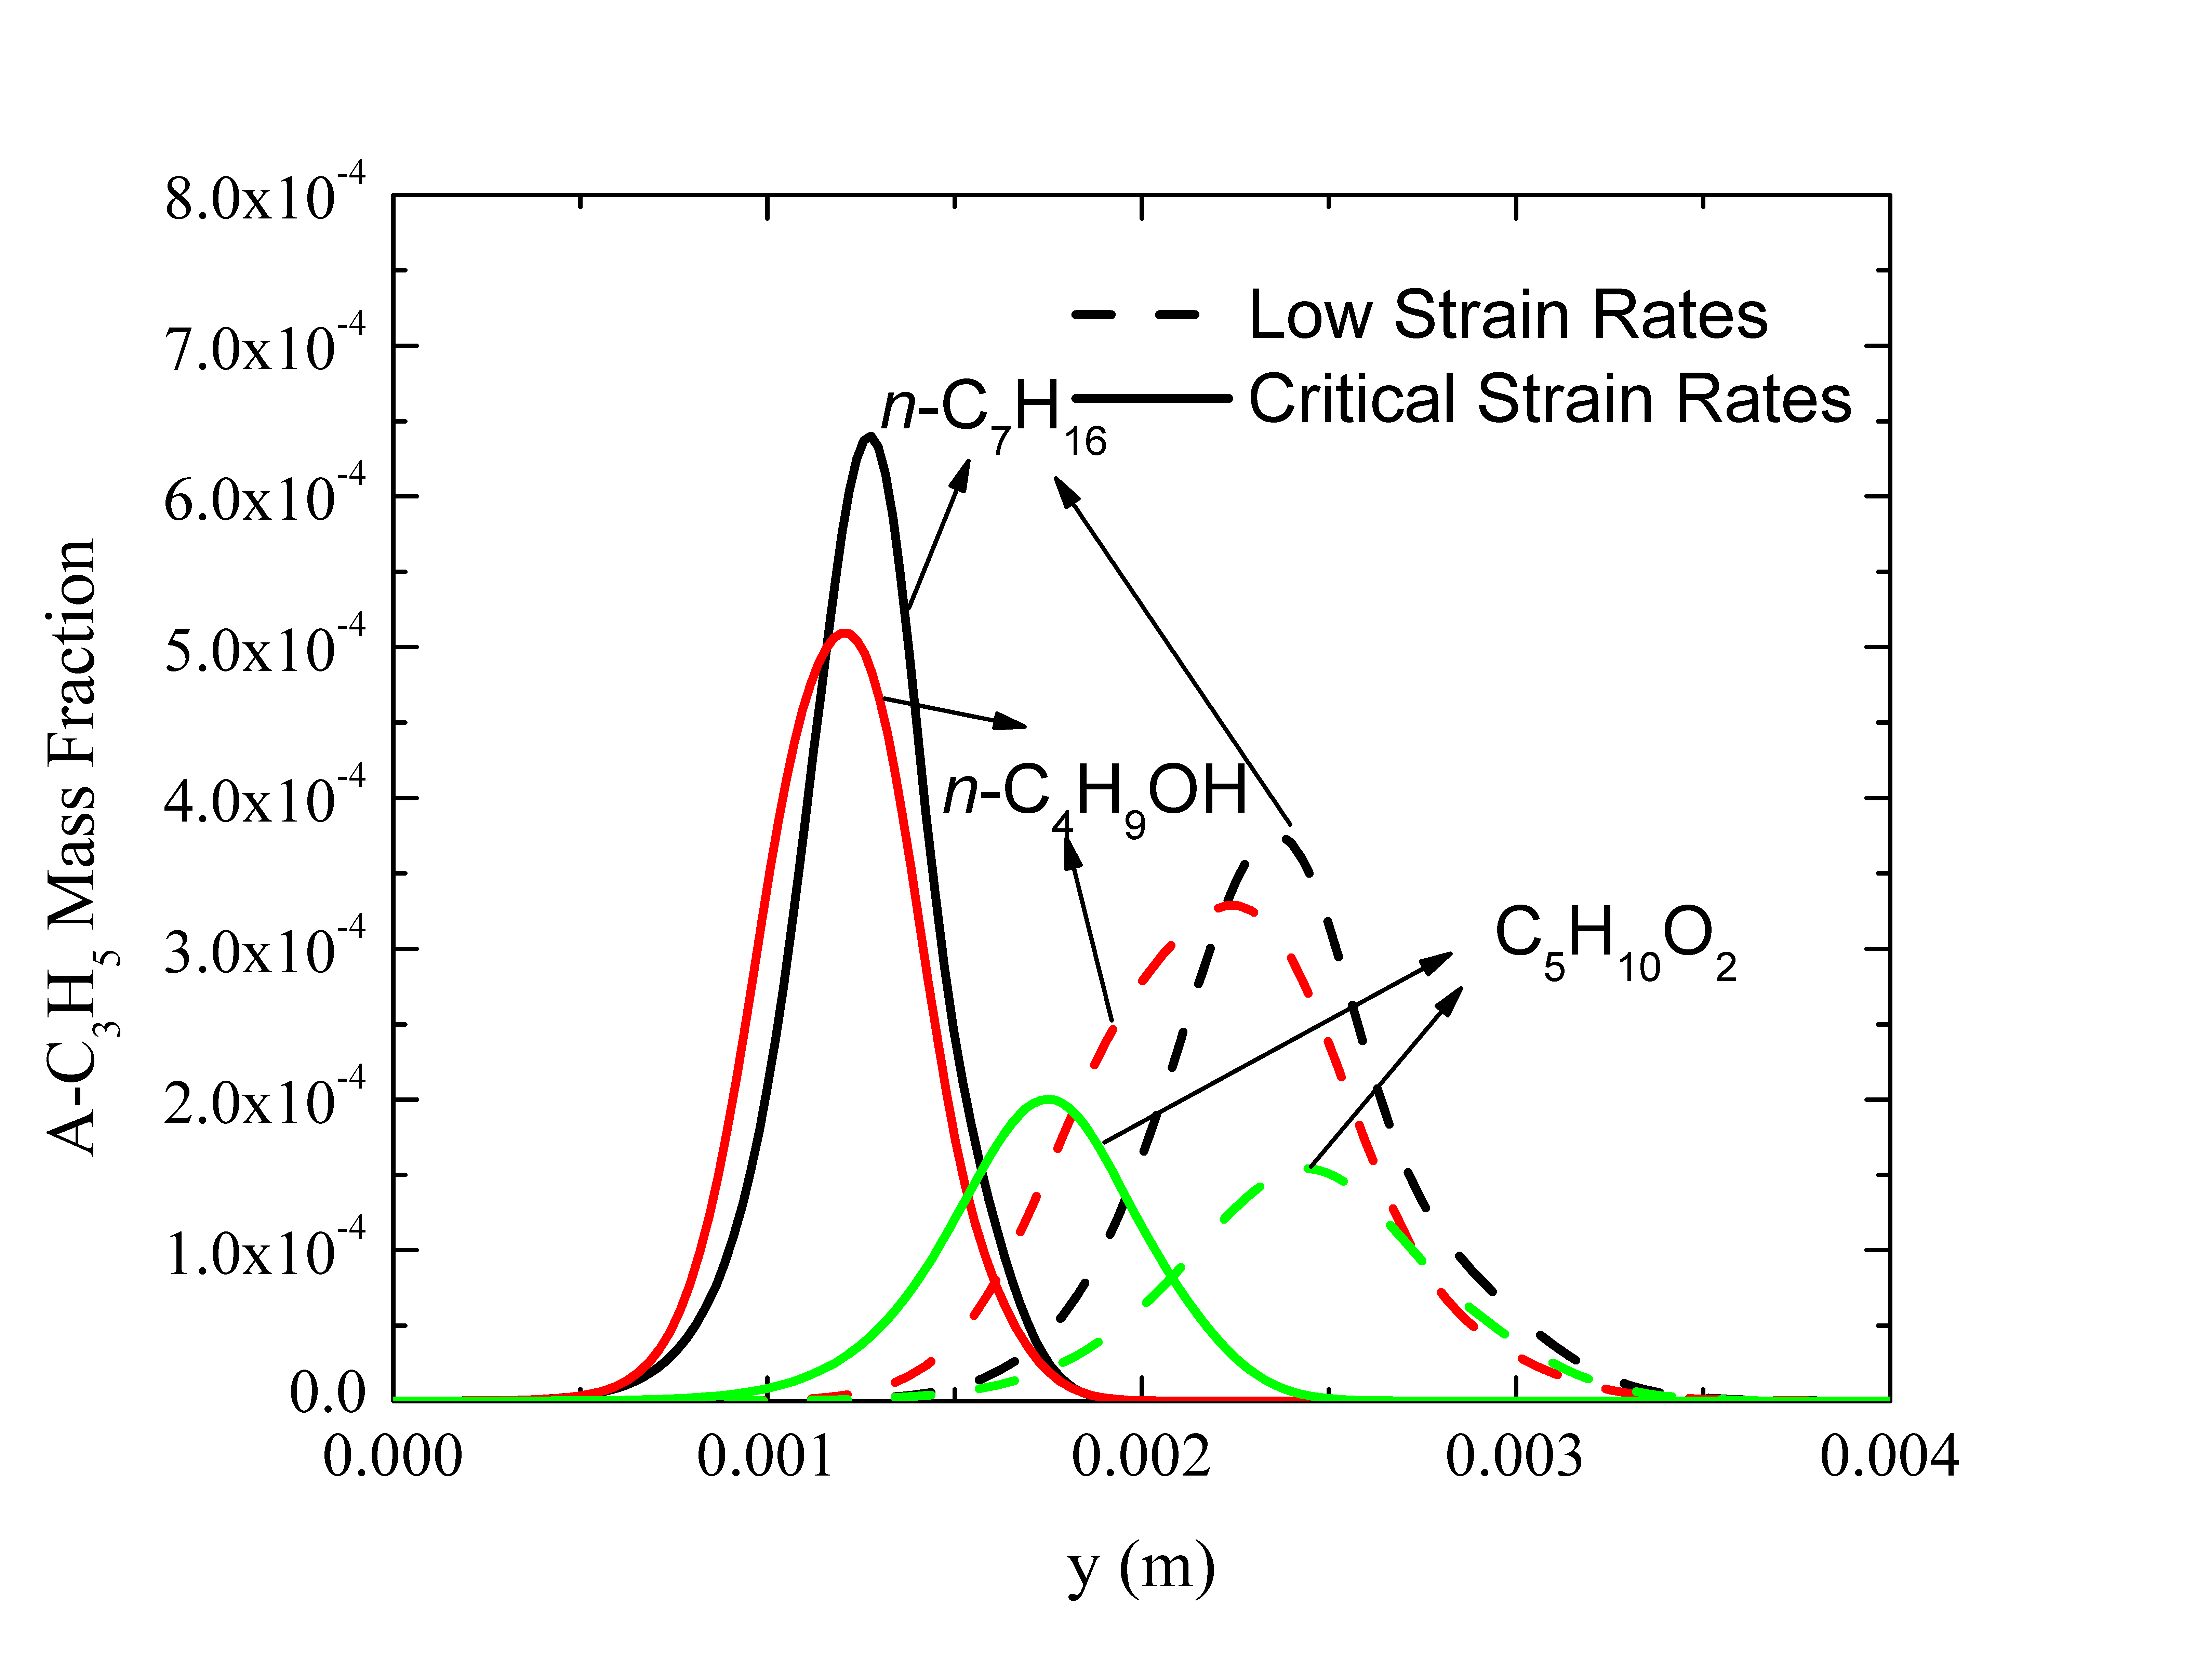
\includegraphics[trim=4mm 8mm 30mm 20mm, clip=true, width=0.48\textwidth]{A-C3H5-y.png}
  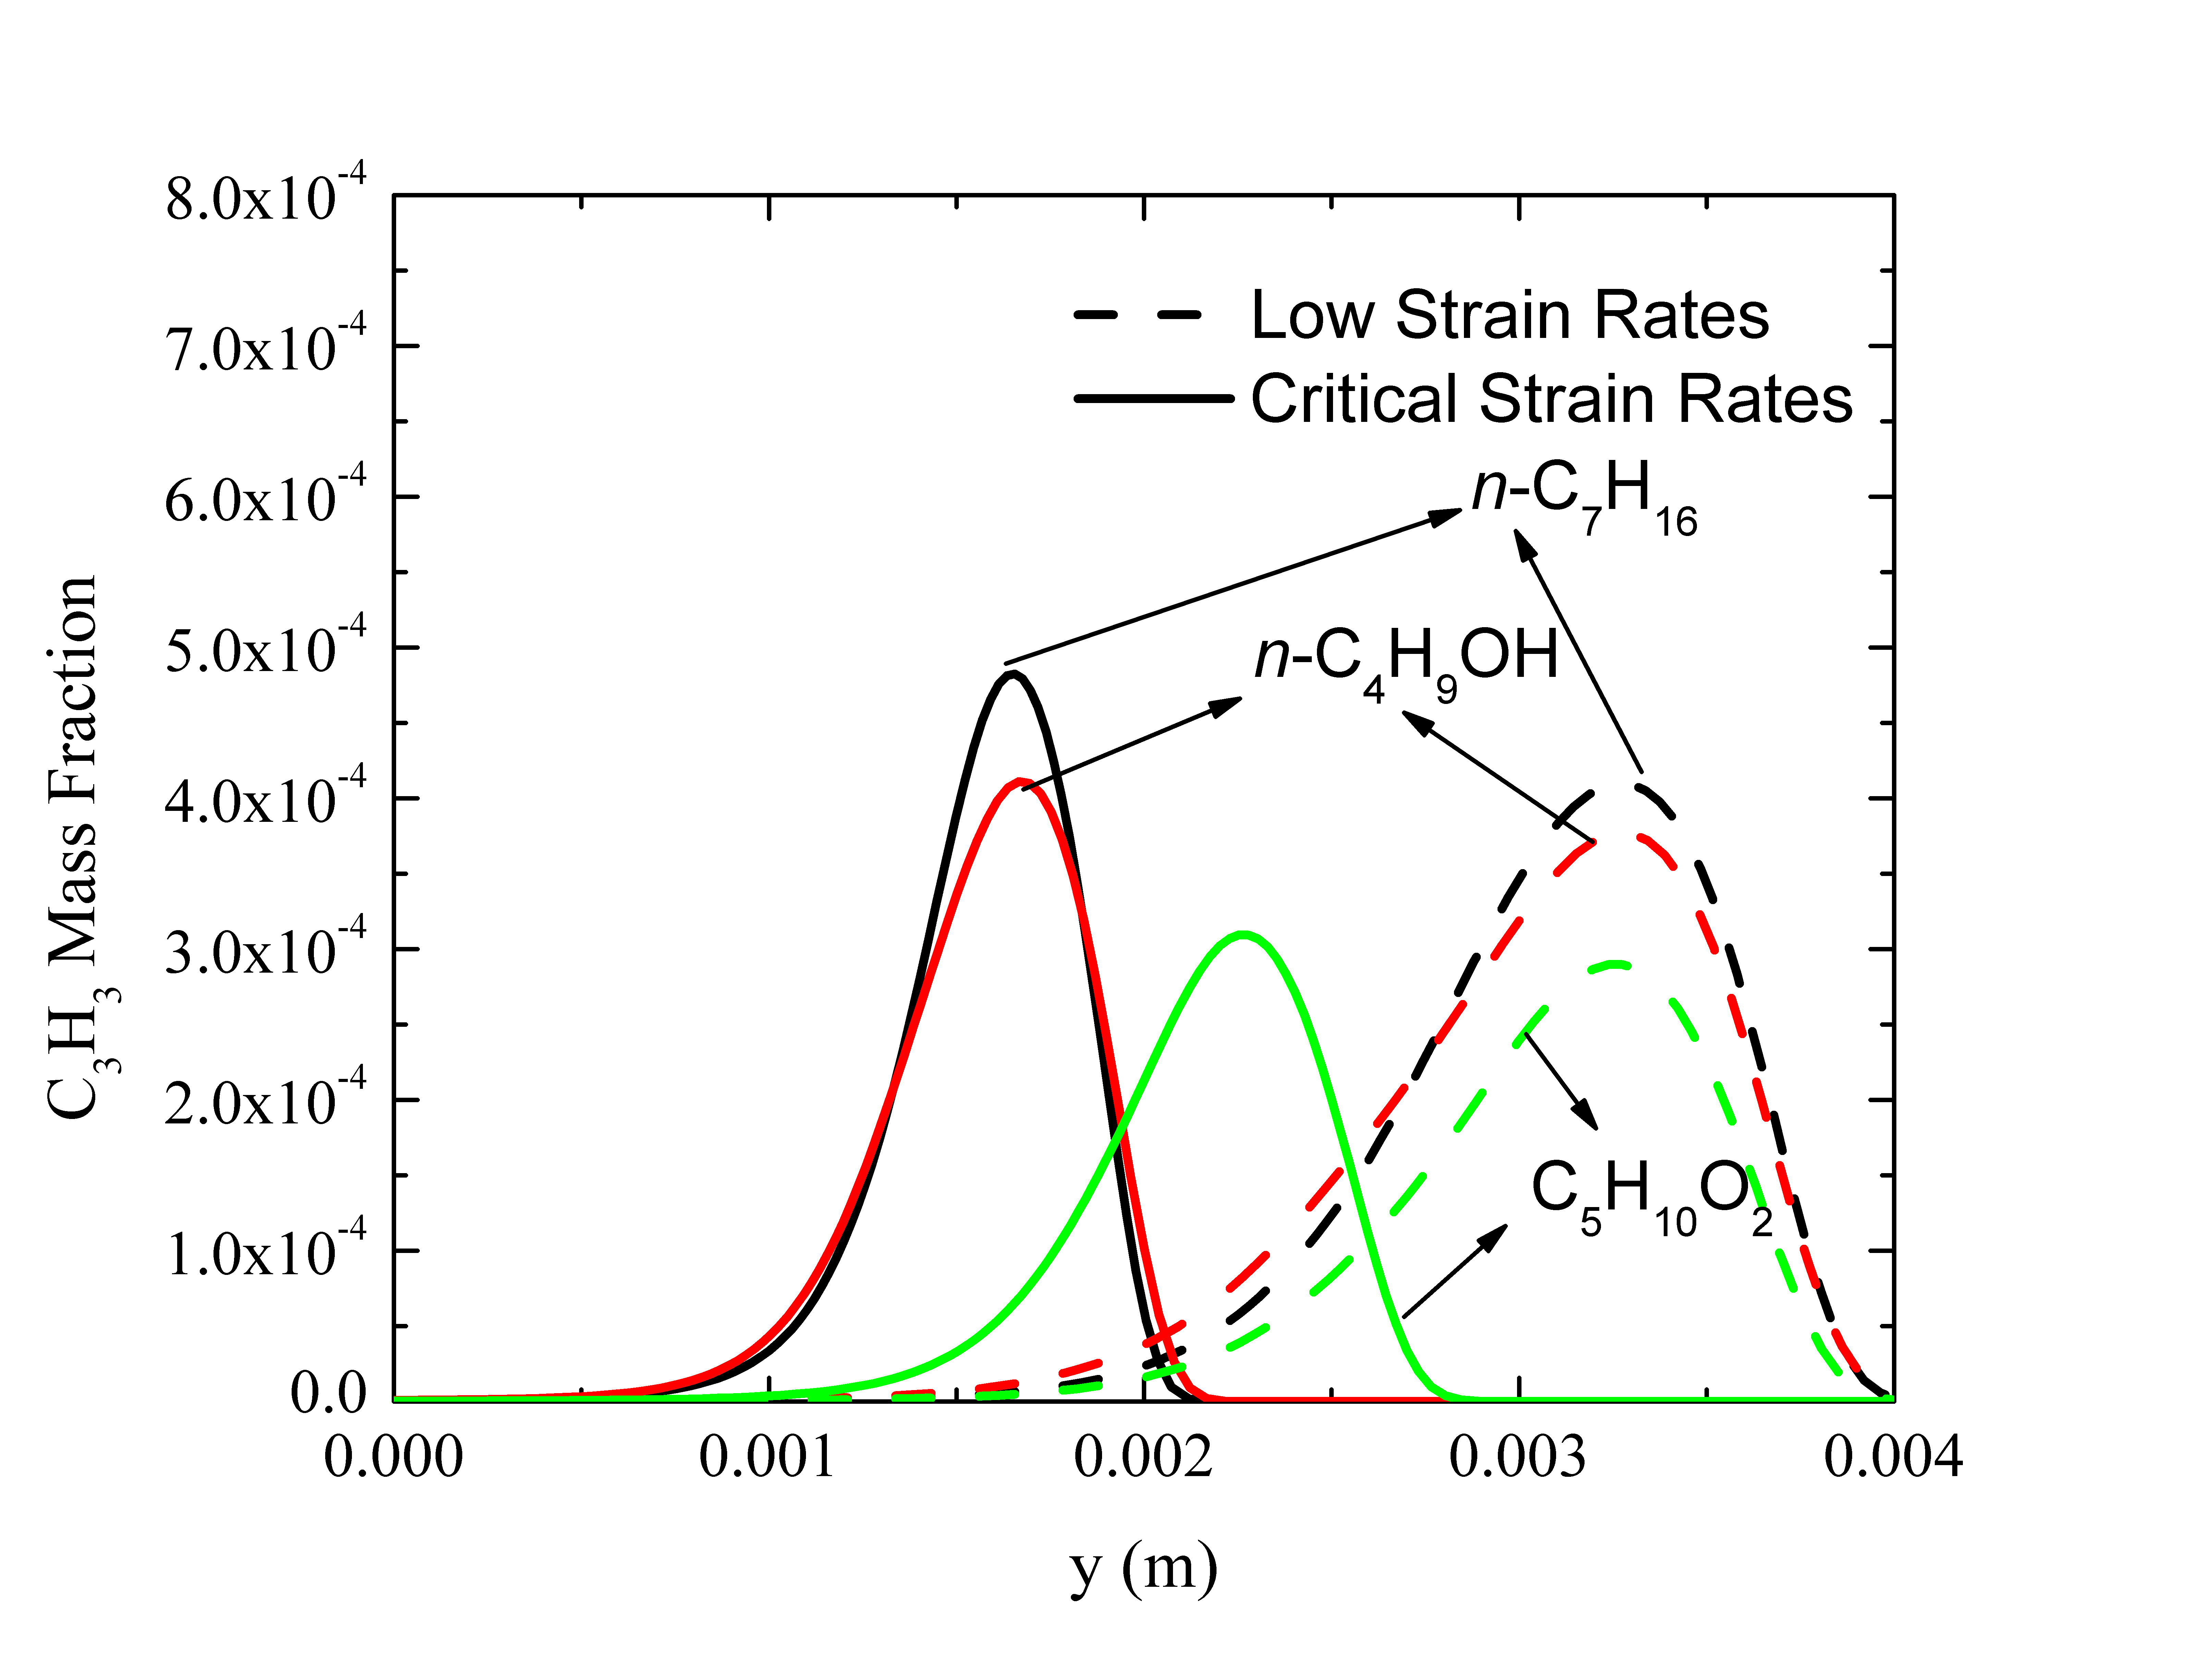
\includegraphics[trim=4mm 8mm 30mm 20mm, clip=true, width=0.48\textwidth]{C3H3-y.png}
  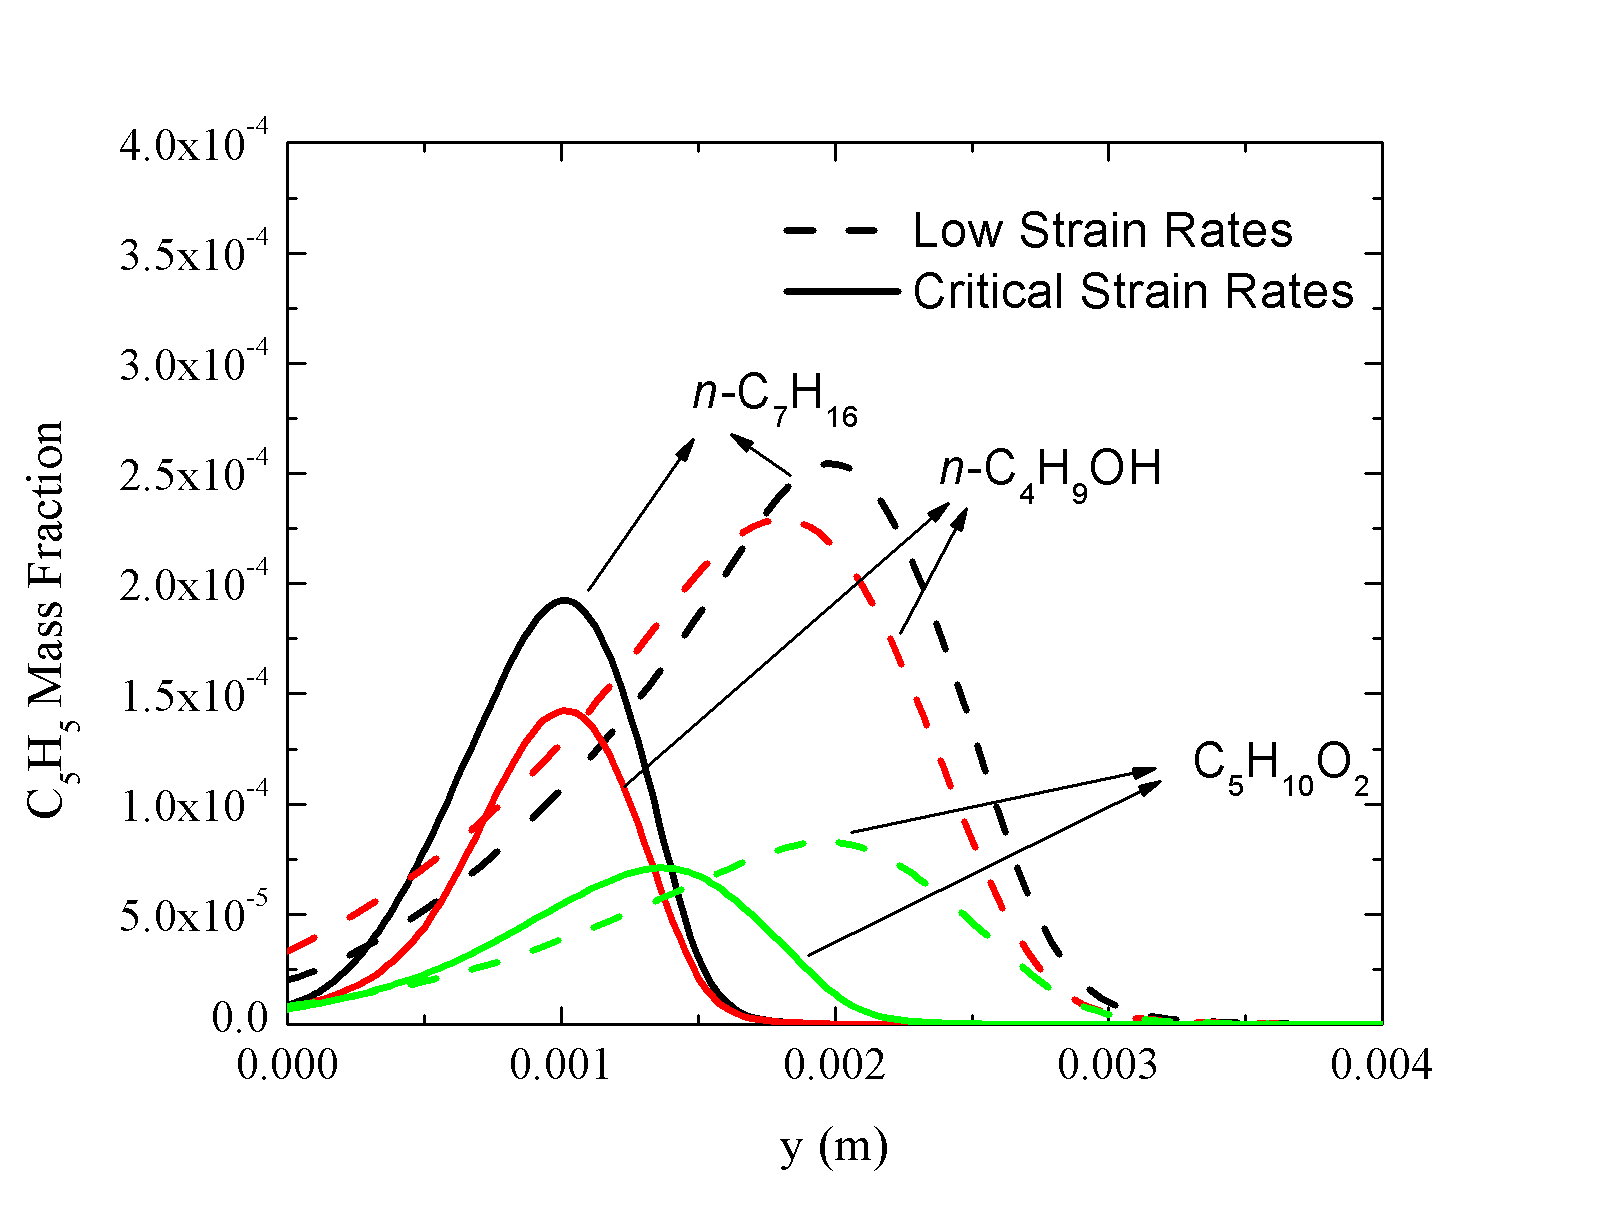
\includegraphics[trim=4mm 8mm 30mm 20mm, clip=true, width=0.48\textwidth]{C5H5-y.png}
  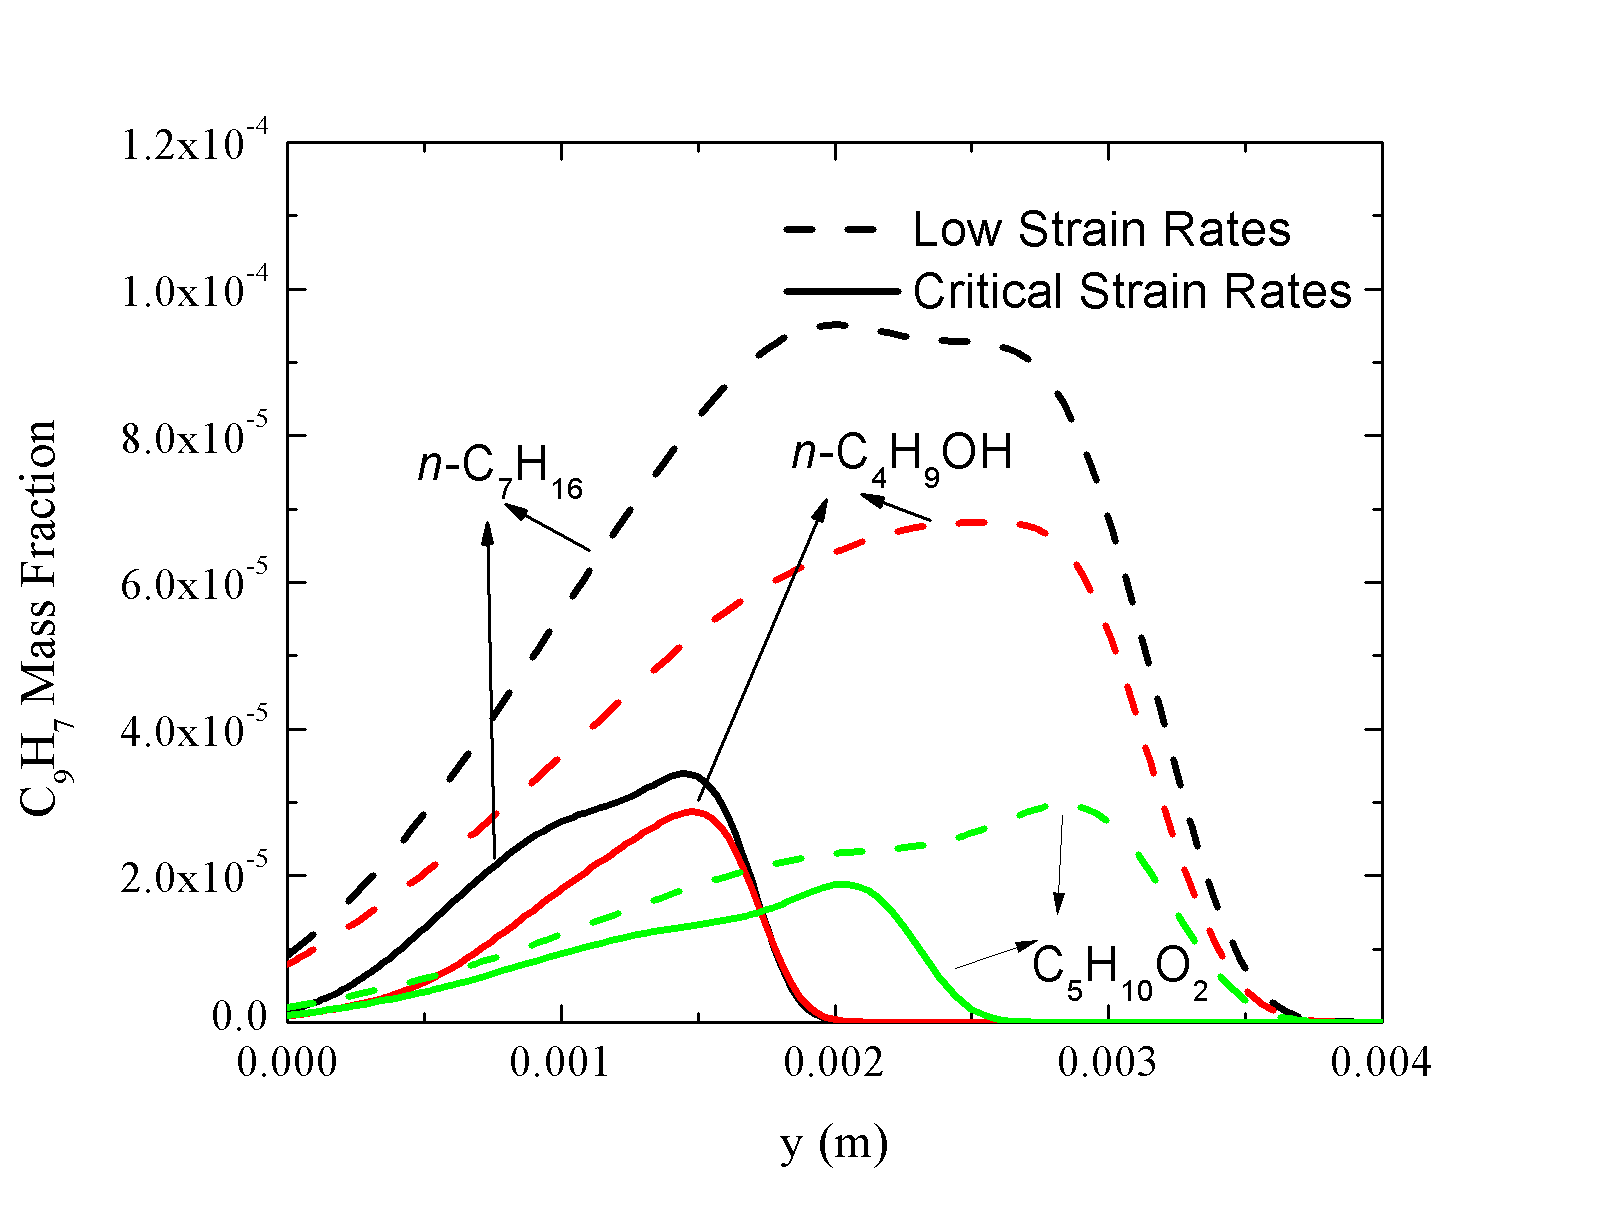
\includegraphics[trim=4mm 8mm 30mm 20mm, clip=true, width=0.48\textwidth]{C9H7-y.png}
  \normalsize
  \vspace{-0.2in}
  \caption{Intermediate species profiles at low strain rates ($16$ s$^{-1}$) and CSRs. $X_{O_2}=0.2$.}
  \label{fig:CxHy}
\end{figure*}


\section{Conclusions}           

In this work, $n$-heptane, $n$-butanol, and methyl butanoate were chosen as diesel/bioalcohol/biodiesel surrogates of interests, due to similar volatilities, thus the potential applications in diesel fuel blending. Their sooting limits were measured experimentally with the stagnation-flow apparatus. Computations were conducted for the same cases using FlameMaster enhanced by the Hybrid Method of Moments (HMOM) soot model with detailed PAH chemistry. Both experimental and computational results show the critical strain rates of the three fuels, based on the absolute soot volume fraction, increase with increasing oxygen mole fraction in the oxidizer, due to the thermal effect. Moreover, although $n$-heptane and $n$-butanol show similar sooting propensities, methyl butanoate is discernibly less sooty.

Sensitivity and reaction path analysis were performed on naphthalene (A2), a typical representative for soot to demonstrate the dependencies of soot formation on gaseous precursors produced by fuel decompositions. It was found that despite different sooting tendencies, the three fuels shared similar PAH chemical pathways. C$_5$, C$_6$, C$_7$, C$_9$ rings and A2 are formed sequentially through the combination of C$_3$ and smaller chain radicals resulted from fuel cracking processes. Due to the fuel bound oxygen in methyl butanoate, less and shorter chain radicals are available for soot formation, compared with the other fuels, such that methyl butanoate has the lowest critical strain rates.

At last, the strain rate effects on soot formation were examined. For all three fuels, C$_5$ and C$_6$ ring formation reactions are the rate limiting steps. Their concentrations drop as the residence time is reduced, such that the downstream PAH chemistry is consequently inhibited, resulting in the sooting limits. 

\section*{Acknowledgments}
TBD

\section*{References}
\bibliographystyle{elsarticle-num}
\bibliography{Soot_m}

\renewcommand{\thefigure}{\arabic{figure}}
\renewcommand{\thetable}{\arabic{table}}

\end{document}

